%%%%%%%%%%%%%%%%%%%%%%%%%%%%%%%%%%%%%%%%%
% Masters/Doctoral Thesis 
% LaTeX Template
% Version 2.2 (21/11/15)
%
% This template has been downloaded from:
% http://www.LaTeXTemplates.com
%
% Version 2.x major modifications by:
% Vel (vel@latextemplates.com)
%
% This template is based on a template by:
% Steve Gunn (http://users.ecs.soton.ac.uk/srg/softwaretools/document/templates/)
% Sunil Patel (http://www.sunilpatel.co.uk/thesis-template/)
%
% Template license:
% CC BY-NC-SA 3.0 (http://creativecommons.org/licenses/by-nc-sa/3.0/)
%
%%%%%%%%%%%%%%%%%%%%%%%%%%%%%%%%%%%%%%%%%

%----------------------------------------------------------------------------------------
%	PACKAGES AND OTHER DOCUMENT CONFIGURATIONS
%----------------------------------------------------------------------------------------
\documentclass[
11pt, % The default document font size, options: 10pt, 11pt, 12pt
%oneside, % Two side (alternating margins) for binding by default, uncomment to switch to one side
spanish, % ngerman for German
singlespacing, % Single line spacing, alternatives: onehalfspacing or doublespacing
%draft, % Uncomment to enable draft mode (no pictures, no links, overfull hboxes indicated)
%nolistspacing, % If the document is onehalfspacing or doublespacing, uncomment this to set spacing in lists to single
%liststotoc, % Uncomment to add the list of figures/tables/etc to the table of contents
%toctotoc, % Uncomment to add the main table of contents to the table of contents
parskip, % Uncomment to add space between paragraphs
%nohyperref, % Uncomment to not load the hyperref package
headsepline, % Uncomment to get a line under the header
]{MastersDoctoralThesis} % The class file specifying the document structure

\usepackage[utf8]{inputenc} % Required for inputting international characters
\usepackage[T1]{fontenc} % Output font encoding for international characters

\usepackage{palatino} % Use the Palatino font by default

%\usepackage[backend=bibtex,style=authoryear,natbib=true]{biblatex} % User the bibtex backend with the authoryear citation style (which resembles APA)
%\addbibresource{example.bib} % The filename of the bibliography
\usepackage[numbers]{natbib}
\usepackage{hyperref}
\usepackage{listings}
\usepackage{array}

\hypersetup{pdfpagemode={UseOutlines},
	bookmarksopen=true,
	bookmarksopenlevel=0,
	hypertexnames=false,
	colorlinks=true, % Set to false to disable coloring links
	citecolor=black, % The color of citations
	linkcolor=black, % The color of references to document elements (sections, figures, etc)
	urlcolor=RoyalBlue, % The color of hyperlinks (URLs)
	pdfstartview={FitV},
	unicode,
	breaklinks=true,
}

\pdfstringdefDisableCommands{% If there is an explicit linebreak in a section heading (or anything printed to the pdf-bookmarks), it is replaced by a space
	\let\\\space%
}

\usepackage{xstring}
\usepackage{todonotes}
\usepackage{pdfpages}
\usepackage{epigraph}
\usepackage{framed}


\let\originalbibitem\bibitem
\def\bibitem#1#2\par{
	\noexpandarg
	\originalbibitem{#1}
	\StrSubstitute{#2}{C.-F. San-Nicolas-Martinez}{\textbf{C.-F. San-Nicolas-Martinez}}\par}
\usepackage[autostyle=true]{csquotes} % Required to generate language-dependent quotes in the bibliography

\addto\captionsspanish{
	\renewcommand{\tablename}{Tabla}
	\renewcommand{\listtablename}{Índice de tablas}
	\renewcommand{\appendixname}{Anexo}
}


%----------------------------------------------------------------------------------------
%	MARGIN SETTINGS
%----------------------------------------------------------------------------------------

\geometry{
	paper=a4paper, % Change to letterpaper for US letter
	inner=3cm, % Inner margin
	outer=2.5cm, % Outer margin
	bindingoffset=0.5cm, % Binding offset
	top=2.5cm, % Top margin
	bottom=2.5cm, % Bottom margin
	%showframe,% show how the type block is set on the page
}
\setlength{\parindent}{8mm}
\setcounter{secnumdepth}{3} % para que ponga 1.1.1.1 en subsubsecciones
\setcounter{tocdepth}{3} % para que ponga subsubsecciones en el indice

%----------------------------------------------------------------------------------------
%----ACRONYMS
%-------------------------------------------------------------------------------------

\begin{document}

\frontmatter % Use roman page numbering style (i, ii, iii, iv...) for the pre-content pages

\pagestyle{plain} % Default to the plain heading style until the thesis style is called for the body content

%----------------------------------------------------------------------------------------
%	TITLE PAGE
%----------------------------------------------------------------------------------------

\begin{titlepage}
	\begin{center}
		UNIVERSIDAD POLITÉCNICA DE CARTAGENA\\
		\vspace*{0.2in}
		\begin{figure}[ht!]
			\centering
			
\includegraphics[width=0.5\linewidth]{imagenes/logoupct.jpg}
		\end{figure}
		ESCUELA TÉCNICA SUPERIOR DE INGENIERÍA DE TELECOMUNICACIÓN\\
		\vspace*{0.35in}
		\begin{large}
			Trabajo Fin de Máster\\
		\end{large}
		\vspace*{0.25in}
		\rule{80mm}{0.1mm}\\
		\vspace*{0.3in}
		\begin{Large}
			\textbf{Desarrollo de APIs para escenarios SDN-NFV} \\
		\end{Large}
		\vspace*{0.35in}
		\rule{80mm}{0.1mm}\\
		\vspace*{0.55in}
	\end{center}
    \vfill
	\begin{flushleft}
		\begin{large}
              \textit{\textbf{Autor:}} César Francisco San Nicolás Martínez\\
			  \textit{\textbf{Director:}} Pablo Pavón Mariño\\
			  \textit{\textbf{Codirector:}} Francisco Javier Moreno Muro\\
		\end{large}
	\end{flushleft}
	\vspace*{0.7in}
	\begin{center}
		FECHA\\
	\end{center}
    \vfill
	
\end{titlepage}
\restoregeometry
\cleardoublepage


\begin{center}
	\vspace*{3cm}
	\fbox{
	\begin{minipage}[][][s]{0.6\linewidth}
		\begin{tabbing}
			\hspace{6.5cm}\=\kill 
			\textbf{Autor:}\>César Francisco San Nicolás Martínez\\ 
			\textbf{E-mail del autor:}\>cesarfsannicolasmartinez@gmail.com\\
			\textbf{Director:} \>Pablo Pavón Mariño \\
			\textbf{E-mail del director:} \> pablo.pavon@upct.es \\
			\textbf{Codirector:} \>Francisco Javier Moreno Muro \\
			\textbf{E-mail de codirector:} \> javier.moreno@upct.es \\
			\textbf{Título del TFM:} \> Desarrollo de APIs para escenarios SDN-NFV\\
		\end{tabbing} 
		\textbf{Resumen:}\\
		El paradigma SDN se ha convertido en una de las maneras más eficientes de gestionar las redes actuales, gracias a la automatización de las funciones de operación y gestión de los diferentes dispositivos de red. A su vez, NFV se ha convertido en un recurso valioso para optimizar recursos de una infraestructura IT. Debido a esto, han ido surgiendo herramientas para la aplicación de las técnicas SDN y NFV. El objetivo de este proyecto es desarrollar diversos clientes para controlar remotamente las herramientas ONOS, OSM y OpenStack e integrarlos en un plugin de la herramienta Net2Plan para realizar una prueba de concepto mediante la interconexión de las diferentes herramientas mencionadas anteriormente.\\

		\begin{tabbing}
			\hspace{6.5cm}\=\kill 
			\textbf{Titulación:}\>Máster en Ingeniería de Telecomunicación\\
			\textbf{Departamento:}\> Tecnologías de la Información y las Comunicaciones \\
			\textbf{Fecha de presentación:}\> FECHA\\
		\end{tabbing} 
	\end{minipage}%
}
\end{center}

\tableofcontents % Prints the main table of contents
%\listoffigures % Print the list of figures


\mainmatter % Begin numeric (1,2,3...) page numbering

\pagestyle{thesis} % Return the page headers back to the "thesis" style

% Include the chapters of the thesis as separate files from the Chapters folder
% Uncomment the lines as you write the chapters
\chapter{Introducción}

El paradigma SDN (\textit{Software Defined Networking}) se ha convertido en una de las maneras más eficientes de gestionar las redes de telecomunicación, permitiendo a los administradores de red una gestión y configuración a alto nivel. Todo esto es gracias a la naturaleza de SDN, cuya principal premisa es la de utilizar un lenguaje común para todos los dispositivos de red, sin importar de que fabricante provengan.

El paradigma NFV (\textit{Network Function Virtualization}) se ha convertido en una de las tecnologías más valiosas para optimizar recursos de una infraestructura IT. Al igual que SDN, NFV permite a los administradores de red la gestión de los recursos; HD, RAM o CPU, entre otros; a alto nivel. Gracias a la naturaleza de NFV, que se basa en la idea de virtualizar cualquier función de red, como puede ser un \textit{firewall} o un dispositivo NAT (\textit{Network Address Traslation}), sustituyendo un dispositivo físico por una máquina virtual que realice su misma función de una manera más eficiente.

Debido a esto, han ido surgiendo herramientas para la aplicación de las técnicas SDN y NFV para automatizar y optimizar las redes de telecomunicación.

\section{Motivaciones}

Este proyecto viene motivado por la evolución de las redes de telecomunicación en los últimos años. El concepto de red de telecomunicación inició como algo puramente físico, constituido exclusivamente por dispositivos \textit{hardware}. Actualmente, una red de telecomunicación está compuesta por dispositivos físicos sustentados por aplicaciones \textit{software} que son utilizadas por los administradores de red para realizar tareas a alto nivel de forma automatizada.

Los paradigmas SDN y NFV han posibilitado esta evolución, permitiendo a los administradores de redes el poder configurar y gestionar una red a un gran alto nivel, así como el sustituir ciertos dispositivos físicos por máquinas virtuales que realicen su misma función dentro de un entorno de red, pero de manera más eficiente.

Para realizar todas estas tareas a alto nivel, son necesarias diferentes herramientas \textit{software} destinadas a tal fin. Cada una de estas herramientas tiene su propia interfaz de comunicación para poder hacer uso de ellas. Un problema que surge es la particularidad de las interfaces de comunicación de las distintas herramientas, ya que cada una de ellas tiene su propia sintáxis.

Así mismo, no existe una entidad central que permita gestionar las interacciones entre las diferentes herramientas de forma óptima. Por esto último surge la idea de desarrollar diferentes clientes \textbf{open-source} para interactuar con las distintas herramientas de una forma sencilla y transparente para el usuario, y convertir a Net2Plan en esa entidad central que se pueda comunicar con las diferentes herramientas y gestionar las interacciones entre ellas.

\section{Objetivos}

El objetivo principal de este trabajo es desarrollar diferentes APIs \textbf{open-source} e integrarlas en un plugin de Net2Plan para llevar a cabo una prueba de concepto. Este objetivo se puede desglosar en otros más pequeños:

\begin{itemize}
	\item Adquisición de conocimientos de las distintas herramientas (ONOS, Mininet, OSM y OpenStack). 
	\item Desarrollo de APIs para entornos SDN (J-ONOS Client).
	\item Desarrollo de APIs para entornos NFV (J-OSM Client y J-OpenStack Client).
	\item Integración de todas las APIs en un plugin de Net2Plan para una prueba de concepto.
	\item Obtención y análisis de resultados.
\end{itemize}

\section{Plan de trabajo}

Para la consecución de los objetivos marcados, el plan de trabajo del proyecto consta de diferentes fases, cada una de ellas destinada a cumplir un objetivo concreto:

\begin{itemize}
	\item Estudio y familiarización con ONOS, Mininet, OSM y OpenStack.
	\item Desarrollo del cliente para interactuar con ONOS (J-ONOS Client).
	\item Desarrollo del cliente para interactuar con OSM (J-OSM Client).
	\item Desarrollo del cliente para interactuar con OpenStack (J-OpenStack Client);
	\item Desarrollo del plugin de Net2Plan integrando los clientes desarrollados.
	\item Realización la prueba de concepto y obtención de resultados.
	\item Análisis de resultados y obtención de conclusiones.
	\item Escritura de la memoria.
\end{itemize}

\clearpage

\section{Estructura de la memoria}

El resto de la memoria de este Trabajo de Fin de Máster se ha estructurado de la siguiente manera:
\begin{itemize}

	
	\item Capítulo 2. Estado del arte
	
	En este capítulo se lleva a cabo una explicación de como herramientas open-source han cambiado el concepto de red de telecomunicación. Así mismo, se realiza una extensa explicación de los paradigmas SDN y NFV.
	
	\item Capítulo 3. Herramientas utilizadas
	
	En este capítulo se realiza una explicación de todas y cada una de las herramientas y librerías que se han utilizado para llevar a cabo este proyecto.
	
	\item Capítulo 4. Desarrollo de APIs
	
	En este capítulo se realiza una explicación de las APIs desarrolladas para este proyecto (J-OSM Client, ONOS Client y OpenStack Client), así como del plugin de Net2Plan diseñado para integrar las APIs mencionadas.
	
	\item Capítulo 5. Prueba de concepto
	
	En este capítulo se lleva a cabo una explicación de las diferentes fases de la prueba de concepto, así como de sus resultados finales.
	
	\item Capítulo 6. Conclusiones
	
	En este capítulo se realiza un análisis de los resultados obtenidos. También se establecen futuras líneas de investigación y desarrollo para dar continuidad al proyecto.
	
	
\end{itemize}
\cleardoublepage
	
 % Terminado (Aplicadas correcciones de Javi)
\chapter{Estado del arte}
En este capítulo se hablará sobre el contexto en el que se enmarca este proyecto, haciendo especial mención a los paradigmas SDN y NFV.

Ambos paradigmas son la base de este Trabajo de Fin de Máster, y por ello se hace una extensa explicación de cada uno de ellos, haciendo mención a sus arquitecturas de trabajo, ya que explican de forma clara y concisa los diferentes elementos que componen dichas arquitecturas y que función desempeñan.

Una vez explicados SDN y NFV, se lleva a cabo una explicación de como han evolucionado las redes de telecomunicación en los últimos años. Esta evolución se debe a la inclusión de herramientas \textit{software}, especialmente las de código abierto, operando junto a los clásicos dispositivos \textit{hardware} para facilitar la configuración, gestión y optimización de la infraestructura de una red de telecomunicación.

\section{SDN}
\label{sec:sdn}

SDN (\textit{Software Defined Networking}) es un paradigma que consiste en una nueva forma de configurar y gestionar las redes de telecomunicación. Su principal premisa es la de separar el plano de control (\textit{Software}) del plano de datos (\textit{Hardware}).

SDN pretende cambiar la manera tradicional de configuración de dispositivos usando instrucciones de bajo nivel por una manera novedosa mediante herramientas \textit{software} a un alto nivel.

SDN surge principalmente por las limitaciones que tienen las tecnologías de redes actualmente. Las dos principales limitaciones son:

\begin{itemize}
	\item \textbf{Dificultad de escalabilidad:} A medida que el tráfico de una red aumenta, la red debe hacer lo mismo. Esto implica nuevos aparatos que deben ser configurados y gestionados. La cantidad de aparatos de una red aumenta de forma exponencial, y ello las hace que la infraestructura de una red sea difícilmente sostenible en cuanto a la configuración y gestión tradicionales.
	
	\item \textbf{Dependencia del fabricante:} Cada fabricante diseña sus dispositivos de red de una manera particular, con su propio sistema operativo y su propia sintaxis de configuración. En una red de telecomunicaciones es habitual que su infraestructura de red esté compuesta por dispositivos de diferentes vendedores y fabricantes, y es necesario conocer a fondo cada uno de los sistemas operativos.
	
\end{itemize}

Una vez identificadas las limitaciones de redes actuales, hay que identificar los beneficios que SDN puede dar a las entidades que opten por esta tecnología en sus redes de telecomunicaciones. Los principales beneficios de SDN son:

\begin{itemize}
	\item \textbf{Reducción del CapEx (\textit{Capital Expenditures}):} CapEx son los costes asociados a bienes físicos. SDN reduce la necesidad de invertir en nuevos bienes físicos (\textit{hardware}), ya que, gracias a su naturaleza, mediante \textit{software} es capaz de reducir notablemente la carga de trabajo de los dispositivos.
	
	\item \textbf{Reducción del OpEx (\textit{Operational Expenditures}):} OpEx son los costes asociados a operaciones y servicios. SDN reduce este tipo de costes debido a su configuración y gestión de los elementos de red mediante \textit{software}. Este control se realiza de forma más sencilla y automática, lo que permite una reducción del tiempo empleado por los administradores de la red.
	
	\item \textbf{Agilidad y flexibilidad:} SDN permite a las diferentes entidades desplegar aplicaciones, servicios e infraestructuras de forma rápida para alcanzar objetivos en el menor tiempo posible.
\end{itemize}

\subsection{Arquitectura SDN}

Las redes definidas por \textit{software} constan de una arquitectura de red específica, compuesta por distintos componentes \textit{hardware} y \textit{software} que interactúan entre sí, como se puede ver en la figura \ref{fig:arquitecturasdn}.
 
\begin{figure}[!ht]
	\centering
	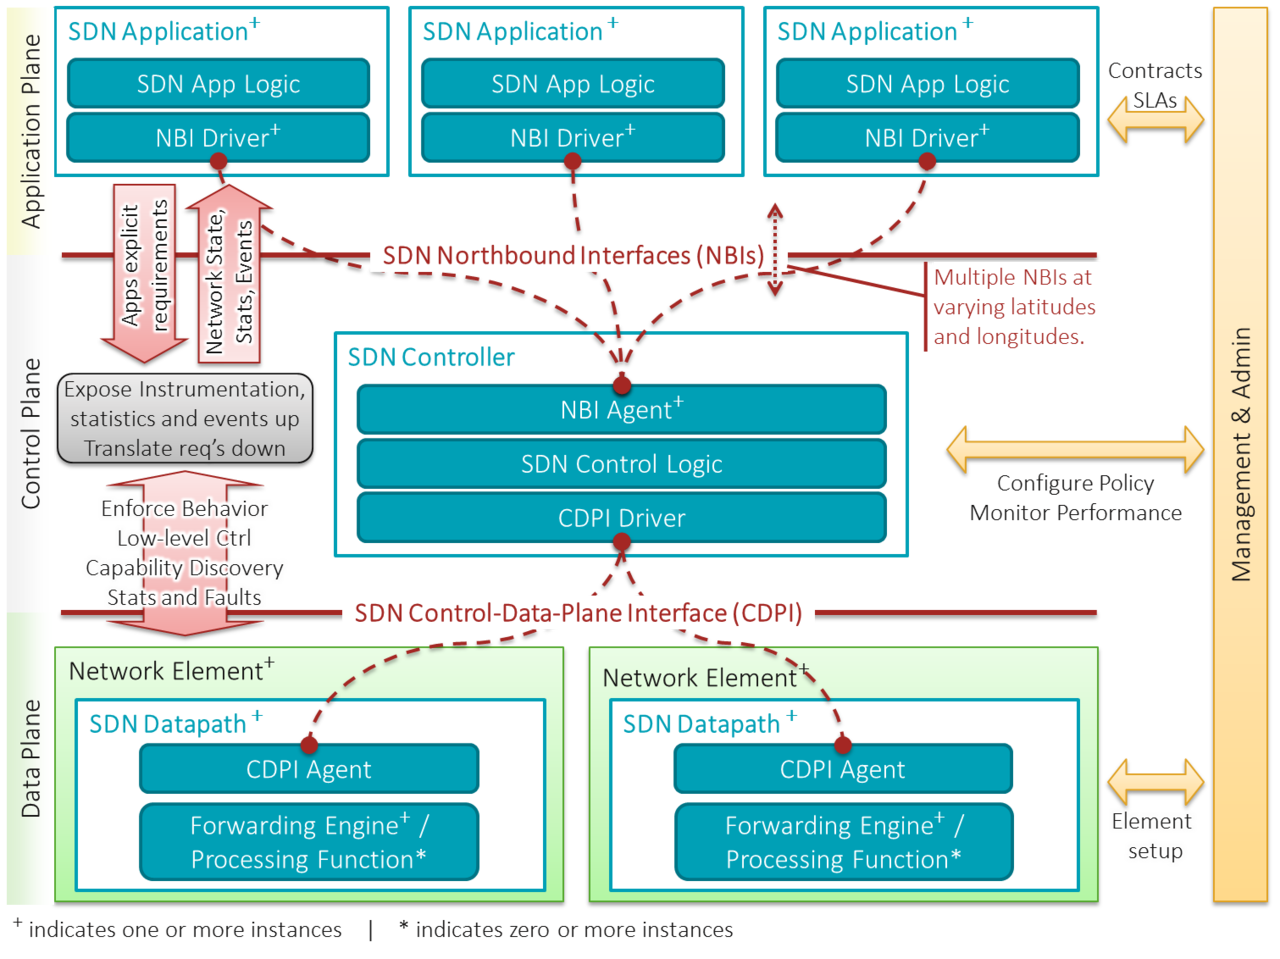
\includegraphics[width=0.75\linewidth]{imagenes/arquitectura_sdn}
	\caption{Arquitectura SDN  Fuente: https://es.wikipedia.org/wiki/Redes\_definidas\_por\_software}
	\label{fig:arquitecturasdn}
\end{figure}

Los diferentes elementos que componen la arquitectura SDN son los siguientes:

\begin{itemize}
	\item \textbf{Controlador SDN:} Es el cerebro de la red SDN. Forma el núcleo de la arquitectura SDN comunicándose con los \textit{switches} a través de la \textbf{Interfaz Sur} (\textit{SouthBound Interface}) y con las distintas aplicaciones a través de la \textbf{Interfaz Norte} (\textit{NorthBound Interface}).
	
	\item \textbf{Interfaz Sur:} Es la interfaz que conecta al controlador SDN con el plano de datos. Facilita la configuración de la red, transfiriendo dichas configuraciones a los dispositivos de la red. El protocolo más utilizado en esta interfaz es \textbf{OpenFlow} (ver \ref{subsec:openflow}).
	
	\item \textbf{Interfaz Norte:} Es la interfaz que conecta al controlador SDN con el plano de control. Facilita el proceso de automatización de la red mediante la comunicación del controlador con las diferentes aplicaciones. Para permitir dicha comunicación con las aplicaciones, la interfaz norte exporta una REST-API.
	
	\item \textbf{Agentes y \textit{Drivers}:} Para establecer la comunicación entre el controlador y los dispositivos mediante la interfaz sur y para la comunicación entre el controlador y las aplicaciones mediante la interfaz norte,es necesario un par agente-\textit{driver}. El \textit{driver} se encuentra en el controlador, mientras que el agente se encuentra en el dispositivo. Se encargan de realizar la comunicación en el plano de datos, realizando la conversión del lenguaje del controlador al del dispositivo, y viceversa.
	
	\item \textbf{Aplicaciones SDN:} Son programas que se conectan al controlador SDN mediante la interfaz norte. Gracias a su lógica de aplicaciones, desarrollan un próposito concreto y transfieren datos u órdenes al controlador SDN.
\end{itemize}


\subsection{OpenFlow}
\label{subsec:openflow}

OpenFlow es un protocolo estándar de SDN, siendo el más utilizado para comunicar el controlador SDN con los dispositivos que se encuentran en el plano de datos. Para que esta comunicación sea posible, el controlador SDN debe tener operando un driver OpenFlow, mientras que el dispositivo debe tener corriendo un agente OpenFlow. 

Un \textit{switch} tradicional utiliza su propia lógica de encaminamiento para decidir como tiene que reenviar los paquetes. Un \textit{switch} OpenFlow es únicamente un dispositivo \textit{hardware} que obedece órdenes que provienen del controlador SDN.

OpenFlow introduce el concepto de flujo, que sustituye a la entrada en la tabla de encaminamiento. Un flujo establece como un \textit{switch} OpenFlow procesa un paquete determinado. Un flujo se compone de dos partes:

\begin{itemize}
	\item \textbf{Selector o regla:} El selector define el conjunto de reglas que debe seguir un determinado paquete. Por ejemplo: tener una dirección MAC origen y/o destino específicas, o una dirección IP origen y/o destino específicas. 
	
	\item \textbf{Tratamiento o acción:} El tratamiento define como se va a procesar un determinado paquete. Por ejemplo: ser reenvíado por un determinado puerto o ser enviado directamente al controlador SDN.
\end{itemize}

Un ejemplo completo de un flujo sería el siguiente:

Todo paquete cuya dirección IP origen sea 10.20.25.45/24 y cuya dirección IP destino sea 10.20.25.46/24, debe ser reenviado por el puerto 3.

\begin{itemize}
	\item El selector es el conjunto de dos reglas que definen al paquete: su IP origen y su IP destino.
	
	\item 	El tratamiento es la orden de reenviar el paquete por el puerto 3.
\end{itemize}
	
A continuación, se empieza ya a hablar más en detalle de un \textit{switch} OpenFlow. Dicho componente tiene las siguientes partes:

\begin{itemize}
	\item \textbf{Agente o Cliente OpenFlow:} Es el encargado de comunicarse con el driver OpenFlow que se encuentra en el controlador SDN.
	
	\item \textbf{Tabla de flujos:} Es la tabla donde se almacenan los flujos del \textit{switch}. Mantiene una relación entre el selector y el tratamiento, así como diferentes estadísticas de monitorización.
	
	\item \textbf{Puerto:} Este concepto es similar al de un \textit{switch} tradicional.
\end{itemize}

\begin{figure}[!ht]
	\centering
	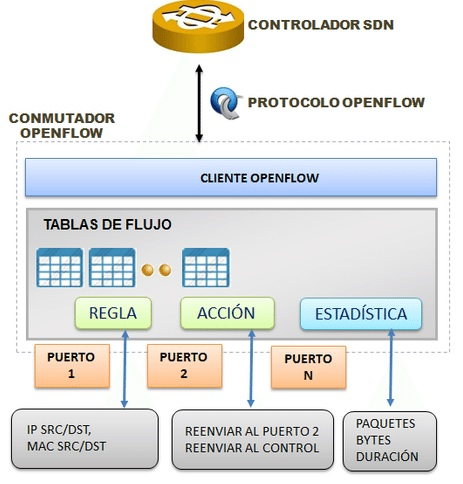
\includegraphics[width=0.7\linewidth]{imagenes/flujosOpenflow}
	\caption{Reglas de flujo en un Switch OpenFlow. Fuente: https://www.researchgate.net/figure/Figura-18-Estructura-y-componentes-de-un-conmutador-OpenFlow-Los-conmutadores-OpenFlow\_fig1\_312187600}
	\label{fig:flujosopenflow}
\end{figure}

\clearpage

En la figura \ref{fig:flujosopenflow} se puede ver la estructura de un \textit{switch} OpenFlow, así como la estructura interna de la tabla de flujos.

Cada vez que un \textit{switch} OpenFlow recibe un paquete, realiza un proceso de \textit{Matching}, es decir, comprueba si el paquete que ha recibido cumple algún selector de su tabla de flujos. Si algún selector coincide con dicho paquete, se reenvía según el tratamiento asociado a dicho selector.

En caso contrario, si dicho paquete no coincide con ninguna entrada de la tabla de flujos, se reenviara por un puerto por defecto, en función de la configuración del propio dispositivo.


\section{NFV}
\label{sec:nfv}

NFV (\textit{Network Function Virtualization}) es un paradigma que engloba a las redes de telecomunicación, más concretamente a su infraestructura. Su principal premisa es la de desacoplar las funciones de red de dispositivos \textit{hardware} y
 trasladarlas a servidores virtuales. Con ello se consigue tener múltiples funciones virtualizadas en un único servidor.

Las redes de telecomunicación actuales tienen ciertos problemas que NFV pretende resolver, como son:

\begin{itemize}
	\item Altos costes y restricciones físicas de fabricación.
	\item Complejidad \textit{hardware} en las soluciones del fabricante.
	\item Ciclo de vida corto de los dispositivos \textit{hardware}.
\end{itemize}

Todos estos problemas o desventajas han desembocado en la adopción de NFV como un estándar para agilizar, facilitar y escalar las infraestructuras de red, así como disminuir costes.

NFV reduce la dependencia de dispositivos \textit{hardware} dedicados. También mejora la escalabilidad y el uso de recursos, ya que una máquina de red puede ser replicada de forma más fácil que un dispositivo físico.

NFV tiene una serie de ventajas importantes que lo convierte en un alternativa óptima:

\begin{itemize}
	\item \textbf{Simplificar la implantación de elementos de red:} Las soluciones de red NFV son flexibles, genéricas y fáciles de implantar, lo que implica que el proceso de actualización es también más rápido y sencillo.
	
	\item \textbf{Mayor escalabilidad de la red:} Gracias a la naturaleza \textit{software} de las funciones virtualizadas, es mucho más fácil escalar los componentes de la red que si se trataran de dispositivos físicos.
	
	\item \textbf{Independencia respecto a los fabricantes de dispositivos:} Debido a que las funciones virtualizadas son desarrolladas mediante \textit{software}, se pierde la dependencia respecto a las particularidades de cada dispositivo, como su sistema operativo o su sintáxis de configuración y gestión, entre otros.
\end{itemize}

\subsection{Arquitectura NFV}
\label{subsec:nfvarq}

La virtualización de funciones de red consta de una arquitectura específica, compuesta por diferentes componentes \textit{hardware} y \textit{software} que interactúan entre sí, como se puede ver en la figura \ref{fig:arquitecturanfv}.

\begin{figure}[!ht]
	\centering
	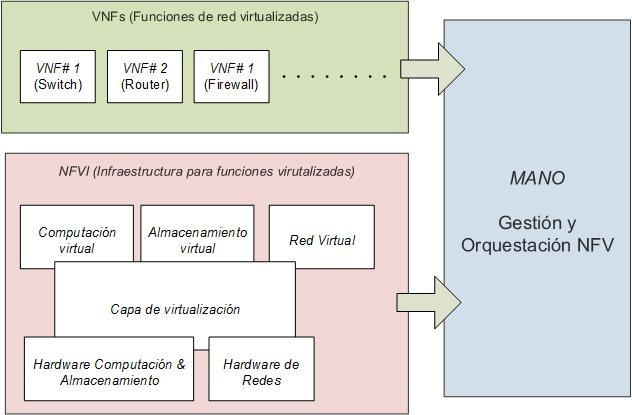
\includegraphics[width=0.75\linewidth]{imagenes/arquitectura_nfv}
	\caption{Arquitectura NFV Fuente: https://es.wikipedia.org/wiki/Virtualización\_de\_funciones\_de\_red}
	\label{fig:arquitecturanfv}
\end{figure}

La arquitectura NFV se compone principalmente de tres componentes, descritos a continuación:

\begin{itemize}
	\item \textbf{Infraestructura NFV:} Es el componente que constituye la base de la arquitectura. Se trata del conjunto de equipos \textit{hardware} y sus recursos (CPU, RAM, HD entre otros) que se utilizan para alojar las máquinas virtuales que componen las diferentes funciones de red virtualizadas (VNFs).
	
	\item \textbf{Bloque de VNFs:} Es el componente que engloba al conjunto de VNFs disponibles para instanciar. Una VNF viene descrita como un conjunto de máquinas virtuales que utilizan determinados recursos de la infraestructura.
	
	\item \textbf{MANO (\textit{Manager and Orchestrator}):} Es el componente que interactúa tanto con la infraestructura NFV. Se encarga de gestionar y orquestar a la propia infraestructura, controlando las acciones que sobre ella se realizan. Dichas acciones pueden ser una nueva instanciación de una VNF o un borrado de una VNF existente, entre otras.
	
\end{itemize}

Después de haber explicado cada uno de los tres componentes de la arquitectura NFV, es necesario poner un ejemplo completo de como se instancia una nueva función de red virtualizada, explicando las interacciones entre los componentes:

\begin{enumerate}
	\item El usuario elige una VNF del bloque de VNFs para instanciar. Dicha orden es transferida al bloque MANO.
	\item El bloque MANO solicita a la infraestructura NFV información sobre sus recursos disponible, para comprobar si la VNF podrá ser instanciada o no.
	\item En caso afirmativo, el bloque MANO recibirá un OK de la infraestructura y procederá a mandar la orden de instanciación.
	\item Una vez enviada la orden de instanciación, la infraestructura NFV reservará los recursos necesarios y arrancará el conjunto de máquinas virtuales pertenecientes a la VNF instanciada.
	\item Si la instanciación ha sido correcta, el bloque MANO recibirá un OK, que será retransmitido al usuario.
	\item El bloque MANO, gracias a su interacción con la infaestructura NFV, proveerá al usuario de datos de monitorización de la VNF instanciada.
\end{enumerate}


\section{Herramientas Open-Source en redes de telecomunicación}
\label{sec:opensourcenets}

Una red de telecomunicación es un conjunto de medios, tecnologías y protocolos que tienen como finalidad el intercambio de información entre diferentes usuarios.

Así mismo, se está produciendo una enorme evolución en el concepto de una red de telecomunicación. 

Antes, este concepto era puramente físico, con un conjunto de dispositivos \textit{Hardware}, como pueden ser \textit{routers}, \textit{switches} u ordenadores, interactuando entre sí. Actualmente, prácticamente el 100\% de las redes utilizan software open-source para diferentes propósitos:

\begin{itemize}
	\item Sacar el máximo rendimiento a su infraestructura.
	\item Agilizar el envío y procesamiento del tráfico de la red.
	\item Acelerar y automatizar la gestión y configuración de los dispositivos.
	\item Reducir los costes de operación de la red.
\end{itemize}

Para conseguir los propósitos mencionados anteriormente, existen numerosas herramientas de software desarrolladas por empresas, universidades u organizaciones que están totalmente disponibles para ser usadas por cualquier usuario.

Dichas herramientas forman un gran conjunto heterogéneo, siendo desarrollada cada una de ellas para uno o más propósitos:

\begin{itemize}
	\item Para sacar el máximo rendimiento a la infraestructura de una red, existen herramientas de virtualización como \textbf{OpenStack} (ver \ref{sec:openstack}) o \textbf{Docker}, para proveer a las aplicaciones de una abstracción e independencia. Este tipo de herramientas se enmarcan dentro de la tecnología \textbf{NFV} (ver \ref{sec:nfv}).
	
	\item Para agilizar el envío y procesamiento del tráfico de una red, existen herramientas que permiten crear dispositivos hardware virtualizados como \textbf{OpenVSwitch} o \textbf{Mininet} (ver \ref{sec:mininet}). Gracias a este tipo de herramientas, se puede sustituir un \textit{Switch} clásico por un pequeño software que hace las funciones de un \textit{Switch} de una manera más eficiente.
	
	\item La gestión de los dispositivos se ha realizado de forma manual, dispositivo a dispositivo. Gracias a herramientas software como \textbf{Cacti} o \textbf{Nagios}, la forma de gestionar las redes de telecomunicación ha dado un giro de 180 grados. Utilizando estas herramientas, el usuario puede gestionar la red desde un terminal de manera remota, gracias al protocolo SNMP (\textbf{Simple Network Management Protocol}).
	
	\item Para acelerar y automatizar la configuración de los dispositivos de una red de telecomunicación, existen herramientas enmarcadas en la tecnología \textit{SDN} (ver \ref{sec:sdn}). Un ejemplo de estas herramientas es el controlador SDN ONOS (ver \ref{sec:onos}).
	
	\item Para reducir los costes de operación de una red, existen herramientas open-source que ayudan a planificar una red de telecomunicación de forma óptima. La más conocida de estas herramientas es \textbf{Net2Plan} (ver \ref{sec:net2plan}), una herramienta de planificación de redes programada en Java.
\end{itemize}

Una vez explicadas las principales herramientas de código abierto que se utilizan en las redes de telecomunicación, hay que hacer un breve inciso en como se relacionan dichas herramientas con SDN y NFV.

\begin{figure}[!ht]
	\centering
	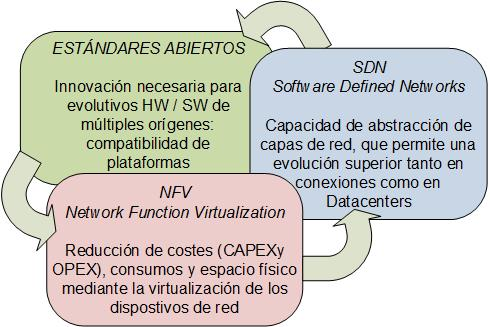
\includegraphics[width=0.75\linewidth]{imagenes/relacionsdnnfv}
	\caption{Relación entre SDN, NFV y las herramientas open-source. Fuente: https://es.wikipedia.org/wiki/Virtualización\_de\_funciones\_de\_red}
	\label{fig:relacionsdnnfv}
\end{figure}

En la figura \ref{fig:relacionsdnnfv} se puede apreciar como los tres conceptos están estrechamente relacionados. 


\cleardoublepage % Terminado a falta de hablar un poco de la relación a 3 bandas (Pulir referencias de fotos)
\chapter{Herramientas utilizadas}

En este capítulo se va a hacer una descripción de cada una de las herramientas utilizadas en el proyecto, haciendo especial mención a Net2Plan, que es la herramienta open-source que ha servido como base para el desarollo de este proyecto..

Por último, se hablará de las diferentes herramientas/aplicaciones que se han utilizado para llevar a cabo este proyecto, como pueden ser ONOS, ETSI-OSM y OpenStack, y de las librerías JAVA que se han empleado para poder realizar la interacción entre todos los componentes.

\section{Net2Plan}
\label{sec:net2plan}

Net2Plan \cite{net2plan} es una herramienta \textit{open-source} programada en Java dedicada a la planificación, optimización y simulación de redes de comunicaciones desarrollada por el grupo de investigación GIRTEL de la Universidad Politécnica de Cartagena. En sus inicios, fue concebida como una herramienta para docencia sobre redes de comunicaciones. Sin embargo, actualmente se ha convertido en una poderosa herramienta de optimización y planificación de redes, con un repositorio de recursos para la planificación de redes, tanto para el entorno académico como para el entorno de la industria y la empresa.

Net2Plan está basado en una representación de redes con componentes abstractos, tales como nodos, enlaces, demandas, ... Ésto está pensado para poder planificar cualquier tipo de red, sin importar la tecnología que utilice. Para poder personalizar las redes a gusto del usuario, cada componentes permite añadir atributos. Además, hay clases que permiten modelar una tecnología en concreto (redes IP, WDM o escenarios de NFV).

Net2Plan tiene dos modos de uso: mediante interfaz gráfica (GUI) y línea de comandos (CLI). La interfaz gráfica está pensada para utilizar en sesiones de laboratorio como un recurso formativo, o para poder ver más detalladamente la red sobre la que se está trabajando. Por otro lado, el modo línea de comandos facilita los estudios de investigación, ya que permite automatizar ejecuciones de algoritmos o simulaciones.
Como se ha hablado antes, ambos modos permiten utilizar Net2Plan en el entorno educativo (investigación o enseñanza) y en el entorno de la industria y la empresa.

\begin{figure}[ht!]
	\centering
	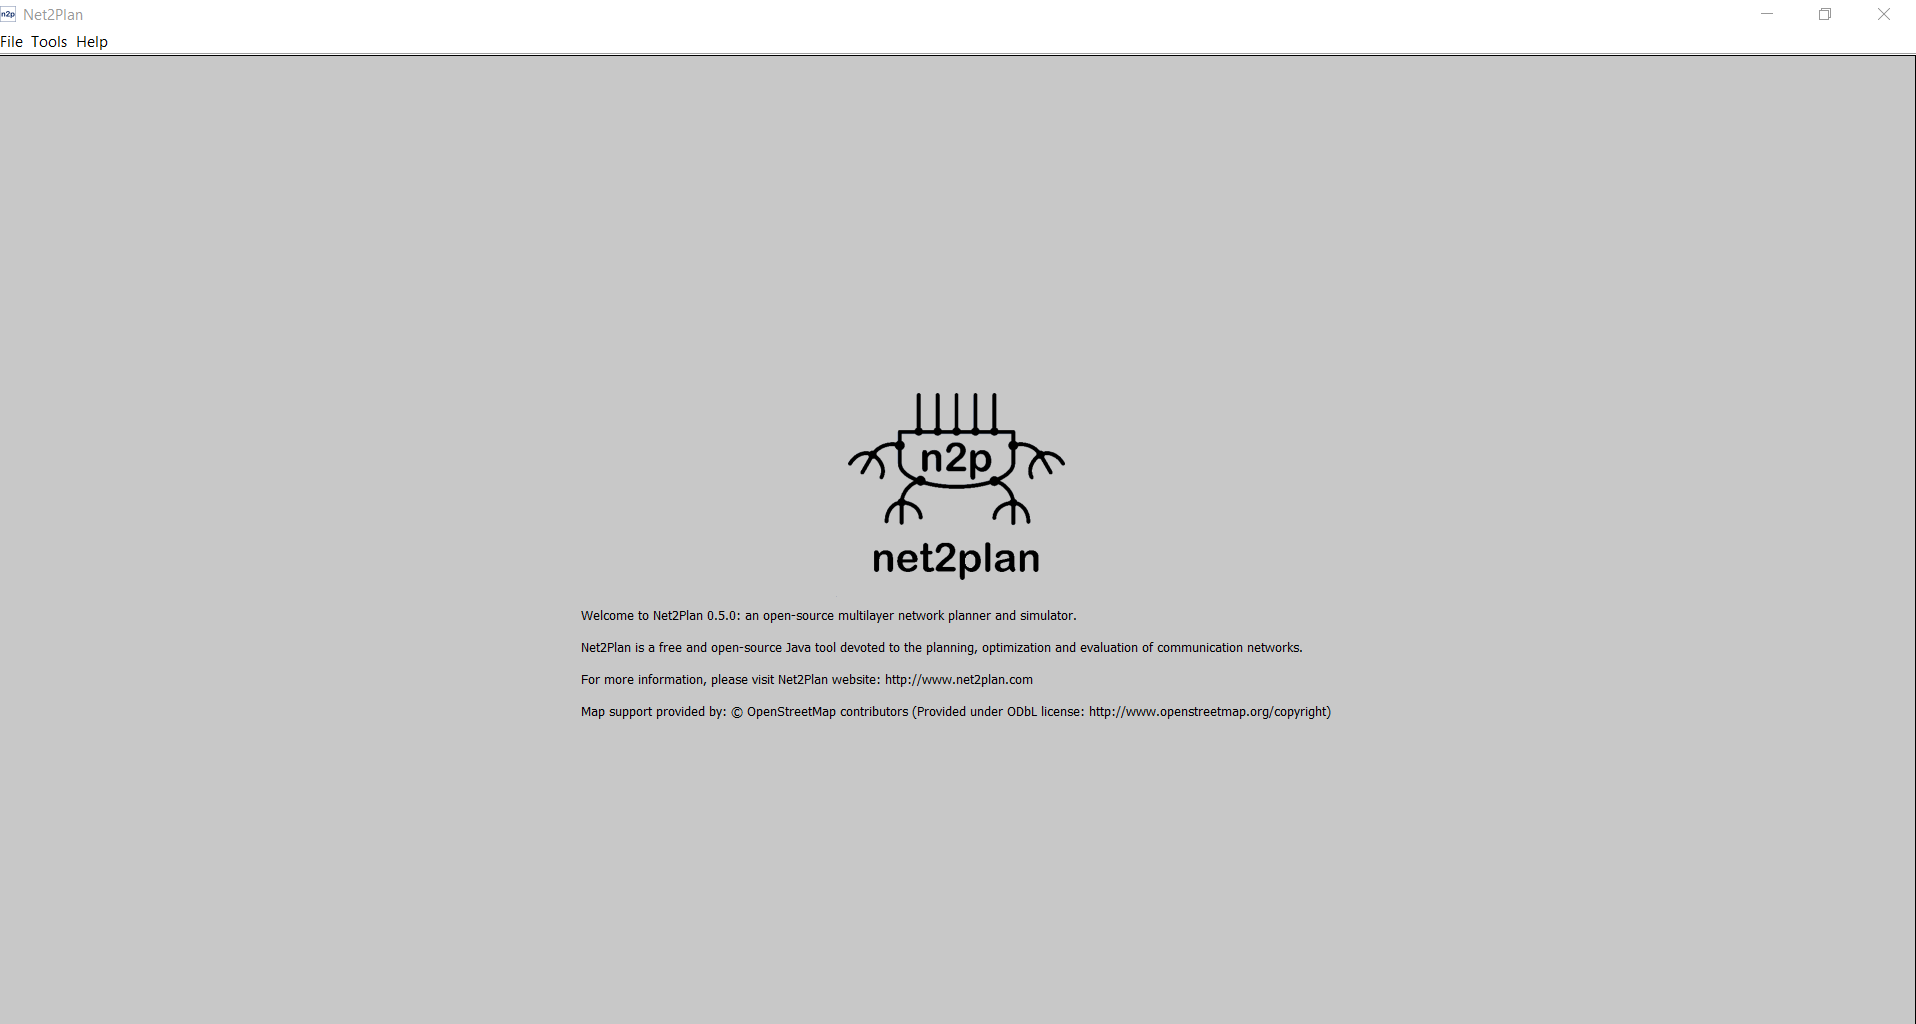
\includegraphics[width=1\linewidth]{imagenes/n2p_inicio}
	\caption{Ventana de inicio de Net2Plan}
	\label{fig:n2p_inicio}
\end{figure}
\begin{figure}[ht!]
	\centering
	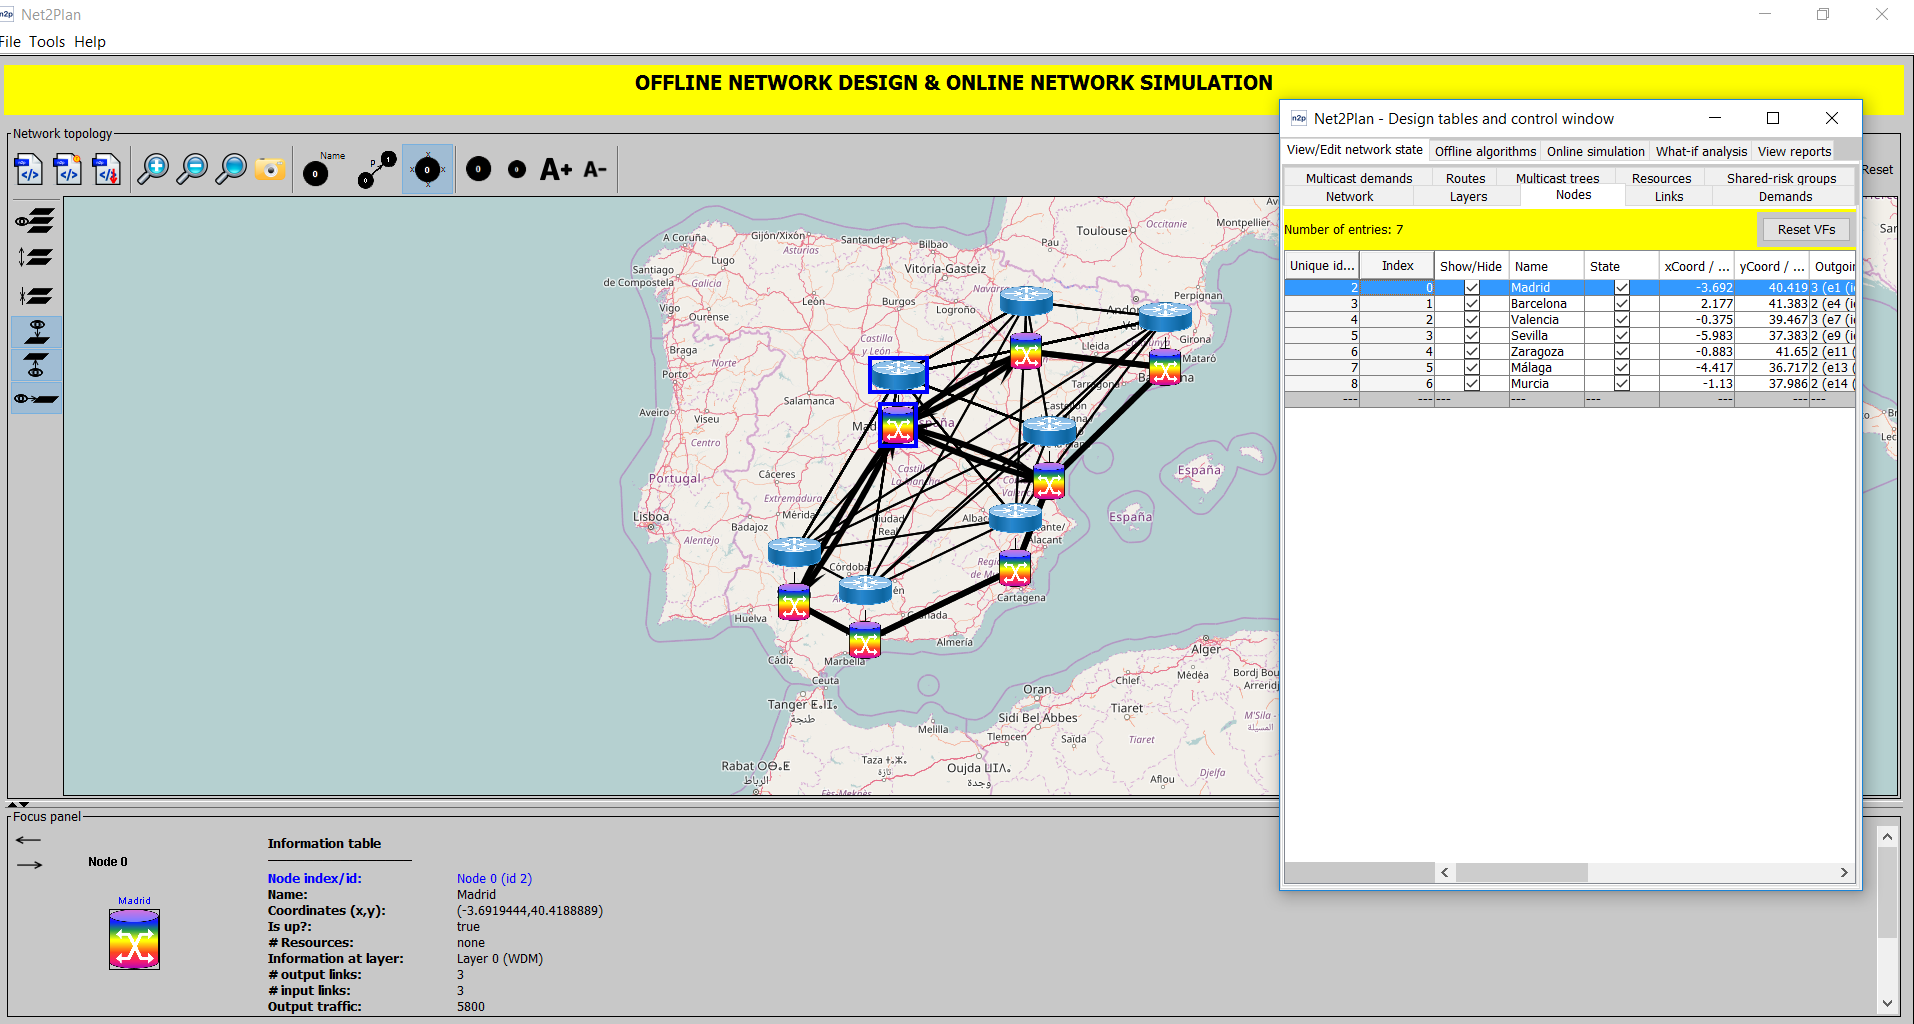
\includegraphics[width=1\linewidth]{imagenes/n2p_redes}
	\caption{Ventana \textit{Offline network desing and online network simulation}}
	\label{fig:n2p_redes}
\end{figure}
\clearpage

\section{Mininet}
\label{sec:mininet}

Mininet es una herramienta de emulación de redes que permite crear redes con \textit{hosts}, \textit{switches}, controladores y enlaces. Los \textit{hosts} de Mininet corren bajo un sistema operativo Linux, mientras que los \textit{switches} soportan el protocolo OpenFlow (ver \ref{subsec:openflow}) para mayor flexibilidad respecto a la configuración del \textit{routing} y para integrarlos dentro de un escenario SDN (ver \ref{sec:sdn}).

Mininet tiene una gran polivalencia, y eso permite que sea utilizado en diferentes tareas, tales como investigación, desarrollo, aprendizaje o testeo. Gracias a ello, se puede conseguir emular una red con un comportamiento similar a una real.

Sus principales características son:
\begin{itemize}
	\item Provee un amplio banco de pruebas para desarrollar aplicaciones basadas en OpenFlow.
	\item Permite que varios desarrolladores trabajen de forma concurrente sobre la misma topología de red.
	\item Permite realizar tests exhaustivos de topologías sin necesidad de tener una real.
	\item Incluye una Interfaz de Línea de Comandos que es independiente de la topología emulada y del protocolo que ésta utilice.
	\item Permite crear desde topologías mas sencillas con un único comando hasta topologías realmente complejas haciendo uso de una API de Python para definir los componentes con total detalle.
\end{itemize}

Las redes emuladas por Mininet ejecutan aplicaciones estandarizadas de Linux, como el kernel del propio sistema Linux. Esto permite que cualquier desarrollo llevado a cabo y testeado en Mininet pueda ser movido a un sistema real realizando las mínimas modificaciones posibles.

\section{ONOS}
\label{sec:onos}

ONOS (Open Network Operative System) es un proyecto Open-Source perteneciente a The Linux Foundation. Su principal objetivo es el de crear un controlador SDN para proveedores de servicios de comunicaciones.

Sus principales características son:
\begin{itemize}
	\item Escalabilidad: Ofrece replicación ilimitada mediante virtualización para poder añadir y quitar capacidad al plano de control según sea necesario.
	\item Alto rendimiento: Se ajusta perfectamente a las especificaciones de los operadores de red.
	\item Resistencia: Provee la disponibilidad requerida por los operadores de red.
	\item Retrocompatibilidad: Permite añadir o configurar dispositivos y servicios con configuración basada en modelos.
	\item Soporte a dispositivos de nueva generación: Ofrece control en real-time para dispositivos OpenFlow y, ahora también para dispositivos P4.
	\item Modularidad: Las funcionalidades de ONOS están definidas en modulos localizados, lo que hace más fácil probar y mantener el software en buen estado.
\end{itemize}


Está escrito en Java y opera como un clúster de nodos idénticos en cuanto al software. Trabaja con modelos y protocolos estandarizados, tales como OpenFlow (ver \ref{subsec:openflow}), NETCONF, OpenConfig, OpenROADM, ...


\begin{figure}[!ht]
	\centering
	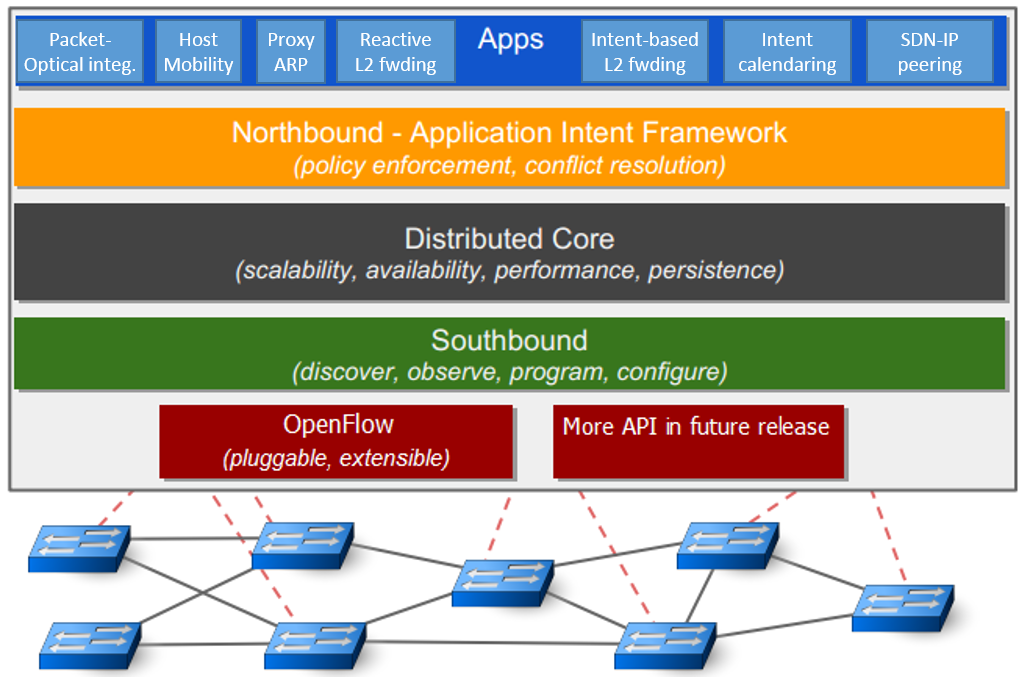
\includegraphics[width=0.6\linewidth]{imagenes/onos_architecture}
	\caption{Arquitectura de ONOS. 
		Fuente: http://sdnhub.org/tutorials/onos/}
	\label{fig:onosarch}
\end{figure}

En la figura \ref{fig:onosarch} se observa la arquitectura interna de ONOS. En el \textit{Core} se encuentran los controladores de los diferentes servicios que ofrece (TopologyService, DeviceService, HostService, ...), cada uno de ellos destinado a controlar un tipo de componente.

También se puede observar que, para acceder a estos controladores, las aplicaciones necesitan hacer uso de la interfaz \textit{NorthBound}, que se compone principalmente de una RestAPI.

Por otro lado, para que los controladores puedan tener constancia de los dispositivos de la red, la interfaz \textit{SouthBound} incluye diferentes \textit{drivers}, genéricos o particulares, para poder comunicarse con dispositivos mediante numerosos protocolos estandarizados, como se explicó anteriormente.

\clearpage

Para facilitar la interacción con el usuario, ONOS ofrece una GUI, como se puede ver en la figura \ref{fig:onosgui}, para ver en más detalle la topología que esta siendo gestionada, así como datos más específicos de cada uno de los dispositivos de la red. 

\begin{figure}[!ht]
	\centering
	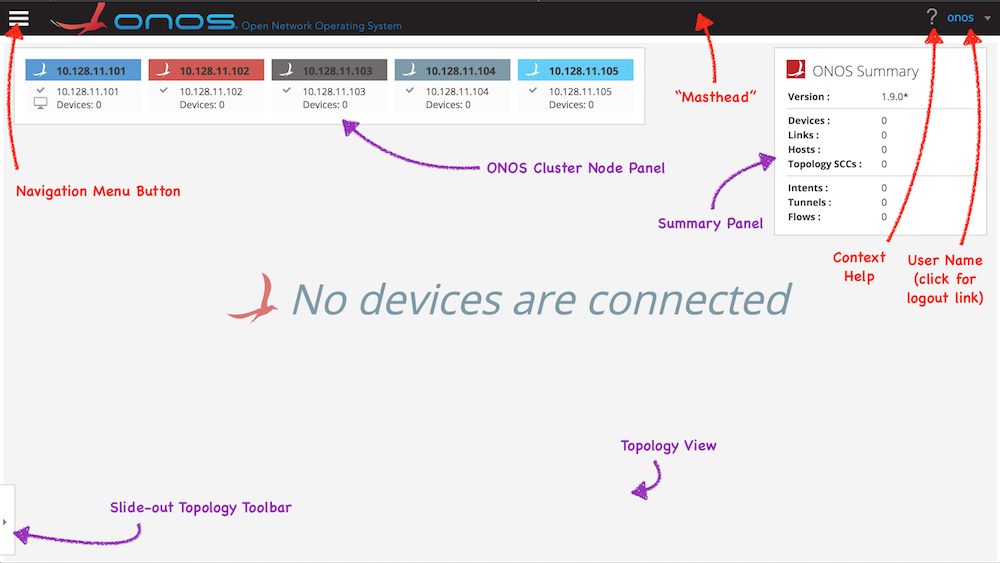
\includegraphics[width=0.8\linewidth]{imagenes/onos_gui}
	\caption{Interfaz Gráfica de ONOS. 
		Fuente: https://wiki.onosproject.org}
	\label{fig:onosgui}
\end{figure}

\subsection{OpenAPI}
\label{subsec:openapi}

OpenAPI es una iniciativa creada por varios expertos de la industria y la investigación para estandarizar las descripciones de las RestAPIs. Su principal objetivo es crear y promover un formato de descripción genérico.

Actualmente, prácticamente todas las aplicaciones utilizar APIs para conectarse con bases de datos, servicios y aplicaciones de terceros,... Gracias a la iniciativa de OpenAPI, las aplicaciones podrán conectarse entre sí de forma más rápida y sencilla, ayudando a tener un mundo realmente comunicado.

\section{OSM}
\label{sec:osm}

OSM (\textit{Open Source MANO}) es un software \textit{open-source} cuya función principal es la orquestación de servicios de red avanzados en infraestructuras NFV heterogéneas. Surge como iniciativa de la ETSI para crear una arquitectura NFV común para los operadores de red.

OSM trabaja con una serie de componentes y conceptos que ayudan a definir su arquitectura:

\begin{itemize}
	\item \textbf{VDU (Virtual Deployment Unit):} Es el componente más básico de la arquitectura OSM. Se encarga de definir una máquina virtual. 
	
	\item \textbf{VLD (Virtual Link Descriptor):} Es el componente que se encarga de definir las conexiones entre diferentes componentes de la arquitectura. Hay principlamente dos tipos de VLD: VDU-VDU y VNF-VNF.
	
	\item \textbf{VNFD (Virtual Network Function Descriptor):} Es el componente que se encarga de definir los recursos necesarios para instanciar un VNF. Incluye diferentes componentes: lista de VDUs, lista de VLDs, lista de conexiones,...
	
	\item \textbf{NSD (Network Service Descriptor):} Es el componente que se encarga de definir la información sobre la configuración de un NS. Incluye diferentes componentes: lista de VNFDs, lista de VLDs, parámetros de configuración iniciales, ...
	
	\item \textbf{VNF (Virtual Network Function):} Es el componente que define una función de red virtualizada. Ésta puede ser completa, cuando es una función realizada únicamente por él, o parcial, cuando es una función mas compleja que requiere de otros VNFs.
	
	\item \textbf{NS (Network Service):} Es el componente que se encarga de agrupar diferentes VNFs que realizan una función de red conjunta.
\end{itemize}

\begin{figure}[!ht]
	\centering
	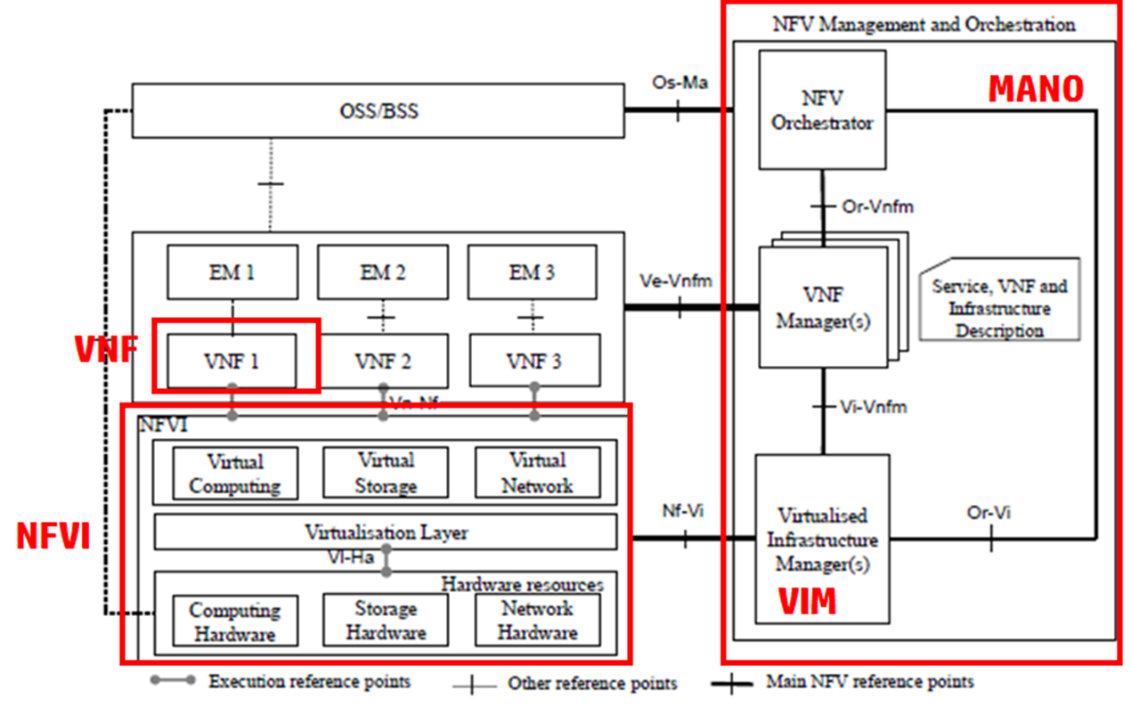
\includegraphics[width=0.8\linewidth]{imagenes/nfv_etsi_Arch}
	\caption{Arquitectura NFV de la ETSI. 
		Fuente: https://sdn.ieee.org/newsletter/july-2016/opensource-mano}
	\label{fig:nfvetsiarch}
\end{figure}

En la figura \ref{fig:nfvetsiarch} se puede ver un esquema de la arquitectura NFV que propone la ETSI, en la que se puede observar el papel que juega OSM en ella. 

\clearpage

\begin{figure}[!ht]
	\centering
	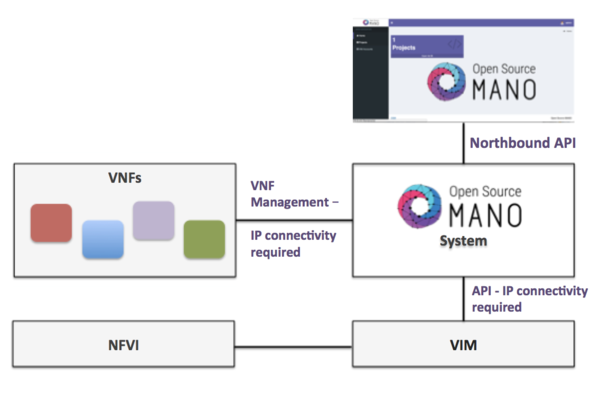
\includegraphics[width=0.8\linewidth]{imagenes/osm_arch}
	\caption{Arquitectura de OSM. 
		Fuente: https://osm.etsi.org/wikipub}
	\label{fig:osmarch}
\end{figure}

Para ayudar a explicar el funcionamiento de OSM, la figura \ref{fig:osmarch} da una visión general de la interaccion entre OSM y los diferentes componentes:

\begin{itemize}
	\item \textbf{Interfaz \textit{NorthBound}:} OSM exporta una RestAPI gracias a su interfaz \textit{NorthBound}. Mediante llamadas HTTP (GET, POST, DELETE), el usuario es capaz de ejecutar órdenes en OSM, tales como crear un nuevo VIM o instanciar un nuevo VNF, entre otras.
	
	Para ello, es necesario tener un cliente desde el cuál enviar órdenes. La ETSI ofrece una interfaz gráfica web que se instala al mismo tiempo que OSM y un cliente por línea de comando escrito en Python (\href{https://osm.etsi.org/wikipub/index.php/OsmClient}{OSMClient}).
	
	\item \textbf{Conexión con VIM:} OSM permite la comunicación con múltiples tipos de VIM (OpenStack, OpenVIM, VMWare y Amazon Web Services). Para ello, es necesaria conectividad IP entre OSM y el propio VIM, ya que las órdenes enviadas por OSM al VIM para realizar operaciones son hechas mediante una RestAPI.
	
	\item \textbf{Conexión VIM-NFVI:} NFV (NFV Infrastructure) es el conjunto de recursos (Memoria RAM, número de CPUs, Memoria de almacenamiento, ...) que son utilizados por un VIM para poder instanciar diferentes máquinas virtuales (VNFs). 
	
	En estructuras de trabajo pequeñas, es habitual que un VIM y su NFVI estén en la misma máquina física, aunque para estructuras reales de trabajo, la NFVI de un VIM puede estar distribuida en diferentes máquinas físicas.
	
	\item \textbf{VNF \textit{Management}:} cuando un VIM instancia un nuevo VNF, se le asigna una dirección IP para poder acceder a la propia máquina virtual y gestionarla. Por ello, es necesario que haya conectividad IP entre OSM y todos los VNFs. 
\end{itemize}

\clearpage

Una vez explicadas las interacciones que realiza OSM, se pueden explicar los pasos que sigue OSM para instanciar un nuevo NS en un determinado VIM:

\begin{itemize}
	\item \textbf{Paso 1.} Mediante la interfaz gráfica de OSM u otro cliente, el usuario escoge el NSD que quiere instanciar y en que VIM quiere hacerlo.
	
	\item \textbf{Paso 2.} OSM se pone en contacto con el VIM para ver si tiene todos los recursos necesarios para poder instanciar el NS.
	
	\item \textbf{Paso 3.} El VIM se pone en contacto con su NFVI para verificar si tiene todos los recursos necesarios. En caso afirmativo, todo continua de forma normal. En caso contrario, el VIM avisará a OSM de que no es posible llevar a cabo la instanciación.
	
	\item \textbf{Paso 4.} Una vez reservados los recursos necesarios, el VIM empieza a instanciar el NS. Esto toma un tiempo, ya que el VIM crea una instancia por VNF y tiene que aplicar todos los parámetros de configuración definidos en los descriptores.
	
	\item \textbf{Paso 5.} Cuando el NS ha sido instanciado satisfactoriamente, el VIM envía a OSM un mensaje de OK y desde OSM ya se pueden gestionar los diferentes VNFs pertenecientes al NS.
\end{itemize}


\section{OpenStack}
\label{sec:openstack}

OpenStack es una arquitectura basada en el paradigma \textbf{Cloud Computing} para controlar y gestionar grandes cantidades de recursos de computación, almacenamiento y red a través de un \textbf{Datacenter}. Para facilitar la gestión de recursos, OpenStack provee al usuario una interfaz gráfica a la vez que también exporta una RestAPI para permitir conectividad con aplicaciones externas.

\begin{figure}[!ht]
	\centering
	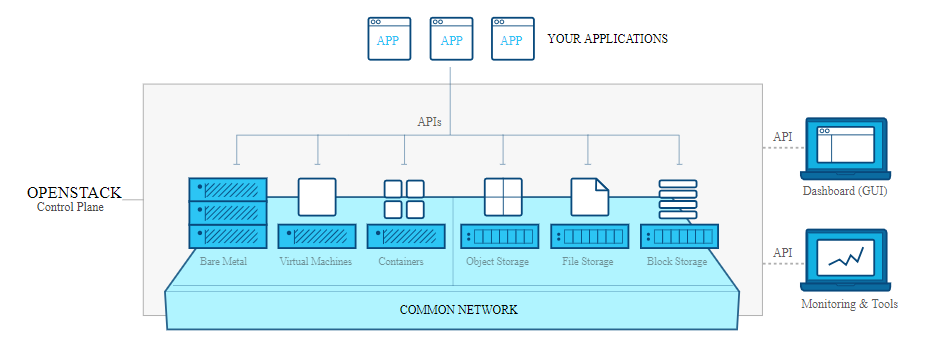
\includegraphics[width=0.9\linewidth]{imagenes/openstack_arch}
	\caption{Arquitectura de OpenStack. Fuente: https://www.openstack.org/software/}
	\label{fig:openstackarch}
\end{figure}

Está compuesto de diferentes servicios o bloques, encargándose cada uno de ellos de una funcionalidad concreta dentro de la arquitectura. Los servicios principales de OpenStack son los siguientes:

\begin{itemize}
	\item \textbf{Keystone:}  Este servicio controla la identificación de los diferentes usuarios que se conecten a la infraestructura de OpenStack, y el acceso a según que aplicaciones de los mismos.
	
	\item \textbf{Horizon:} Este servicio es el encargado de mostrar la gestión completa de OpenStack mediante una interfaz gráfica. Desde ella se puede observar con todo detalle que está sucediendo en el sistema y poder gestionar los posibles fallos.
	
	\item \textbf{Nova:} Este servicio está considerado el motor de OpenStack. Es el encargado de desplegar y administrar las diferentes máquinas virtuales instanciadas y otros servicios que se necesiten.
	
	\item \textbf{Neutron:} Este servicio es el encargado de que cada componente desplegado en OpenStack se comunique con los demas y estén interrelacionados.
	
	\item \textbf{Glance:} Este servicio se encarga de gestionar las diferentes imágenes que se usan en la infraestructura.
	
	\item \textbf{Cinder:} Este servicio se centra en el almacenamiento. Facilita el acceso al contenido alojado en las unidades de disco que se encuentren en la infraestructura.
	
	\item \textbf{Swift:} Este servicio es el encargado de almacenar los diferentes archivos del sistema, asegurar su integridad y replicarlos por los diferentes discos de la infraestructura, para hacer más dinámicas la accesibilidad y la disponibilidad.
\end{itemize}

\subsection{OpenStack4j}
\label{subsec:openstack4j}

OpenStack4j es una librería REST \textit{open-source} programada en Java para controlar y gestionar un sistema basado en OpenStack.

Permite al usuario realizar una gestión de OpenStack eficiente gracias a sus múltiples módulos, cada uno de ellos focalizado en gestionar un servicio concreto de OpenStack:

\begin{itemize}
	\item \textbf{Identity:} Este módulo se encarga de gestionar el servicio \textbf{Keystone}. Su principal objetivo es el de gestionar el directorio de usuarios, grupos, regiones, servicios y \textbf{endpoints}. Así mismo, se encarga de autenticar y autorizar a los diferentes usuarios para utilizar los diferentes servicios.
	
	\item \textbf{Compute:} Este módulo se encarga de gestionar el servicio \textbf{Nova}. Es el encargado de gestionar las diferentes máquinas virtuales que están corriendo en OpenStack.
	
	\item \textbf{Network:} Este módulo se encarga de gestionar el servicio \textbf{Neutron}. Provee conectividad entre diferentes componentes de OpenStack. Permite a los usuarios crear sus propias redes y añadirles interfaces.
	
	\item \textbf{Image:} Este módulo se encarga de gestionar el servicio \textbf{Glance}. Su principal funcionalidad es la de proveer diferentes servicios para la gestión de imágenes. Permite almacenar imágenes personalizadas por el usuario para inicializar máquinas rápidamente.
	
	\item \textbf{Block Storage:} Este módulo se encarga de gestionar el servicio \textbf{Cinder}. Permite al usuario crear y montar volúmenes para escalar el almacenamiento.
	
	\item \textbf{Object Storage:} Este módulo se encarga de gestionar el servicios \textbf{Swift}. Es el encargado de crear almacenamiento persistente para los diferentes archivos alojados en el sistema.
\end{itemize}

En la figura \ref{fig:ejemploos4j} se puede ver un breve ejemplo de como utilizar los servicios Identity, Compute, Image y Network.

\begin{figure}[!ht]
	\centering
	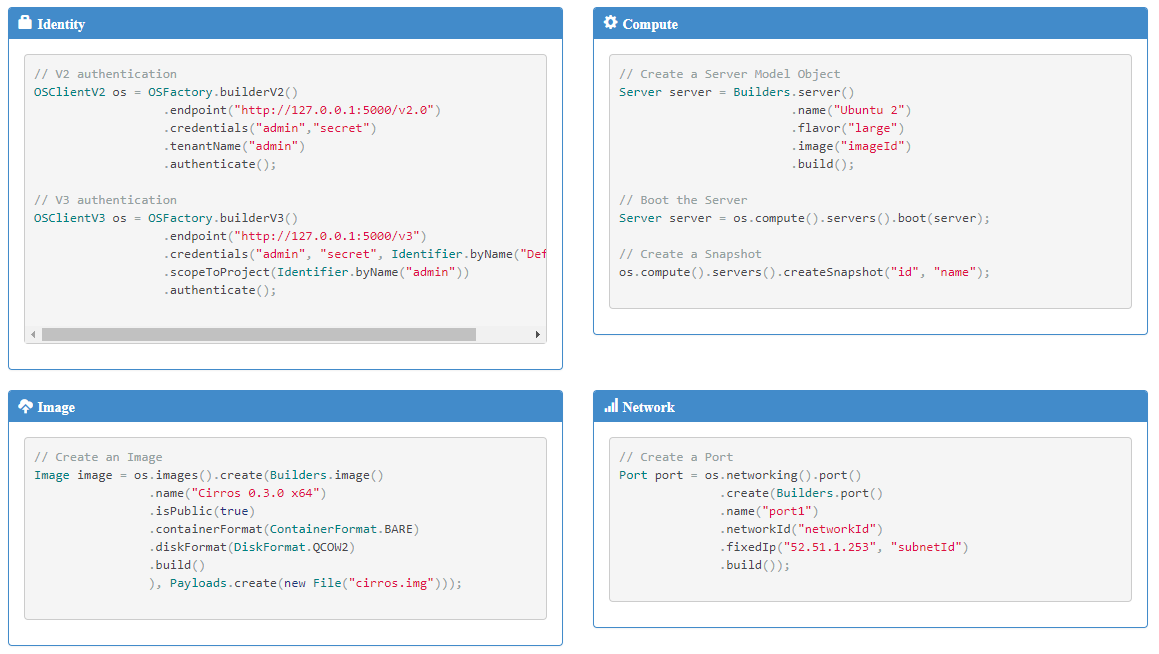
\includegraphics[width=0.8\linewidth]{imagenes/ejemplo_os4j}
	\caption{Ejemplo de uso de OpenStack4j. Fuente: http://www.openstack4j.com/}
	\label{fig:ejemploos4j}
\end{figure}


\cleardoublepage
 % Terminado (Pulir referencias de fotos)
\chapter{Desarrollo de APIs}

En este capítulo se hablará sobre las diferentes librerías (APIs) que se han realizado en este proyecto, explicando detalladamente la estructura de cada una de ellas.

Por último, se hará especial énfasis en el plugin de Net2Plan desarrollado, en el cual se han integrado las difrentes APIs mencionadas anteriormente.


\section{J-OSM Client}
\label{sec:osmclient}

J-OSMClient es una librería programada en Java cuya funcionalidad es la de proporcionar un cliente REST para interactuar con OSM (ver sección \ref{sec:osm}).

\begin{figure}[!ht]
	\centering
	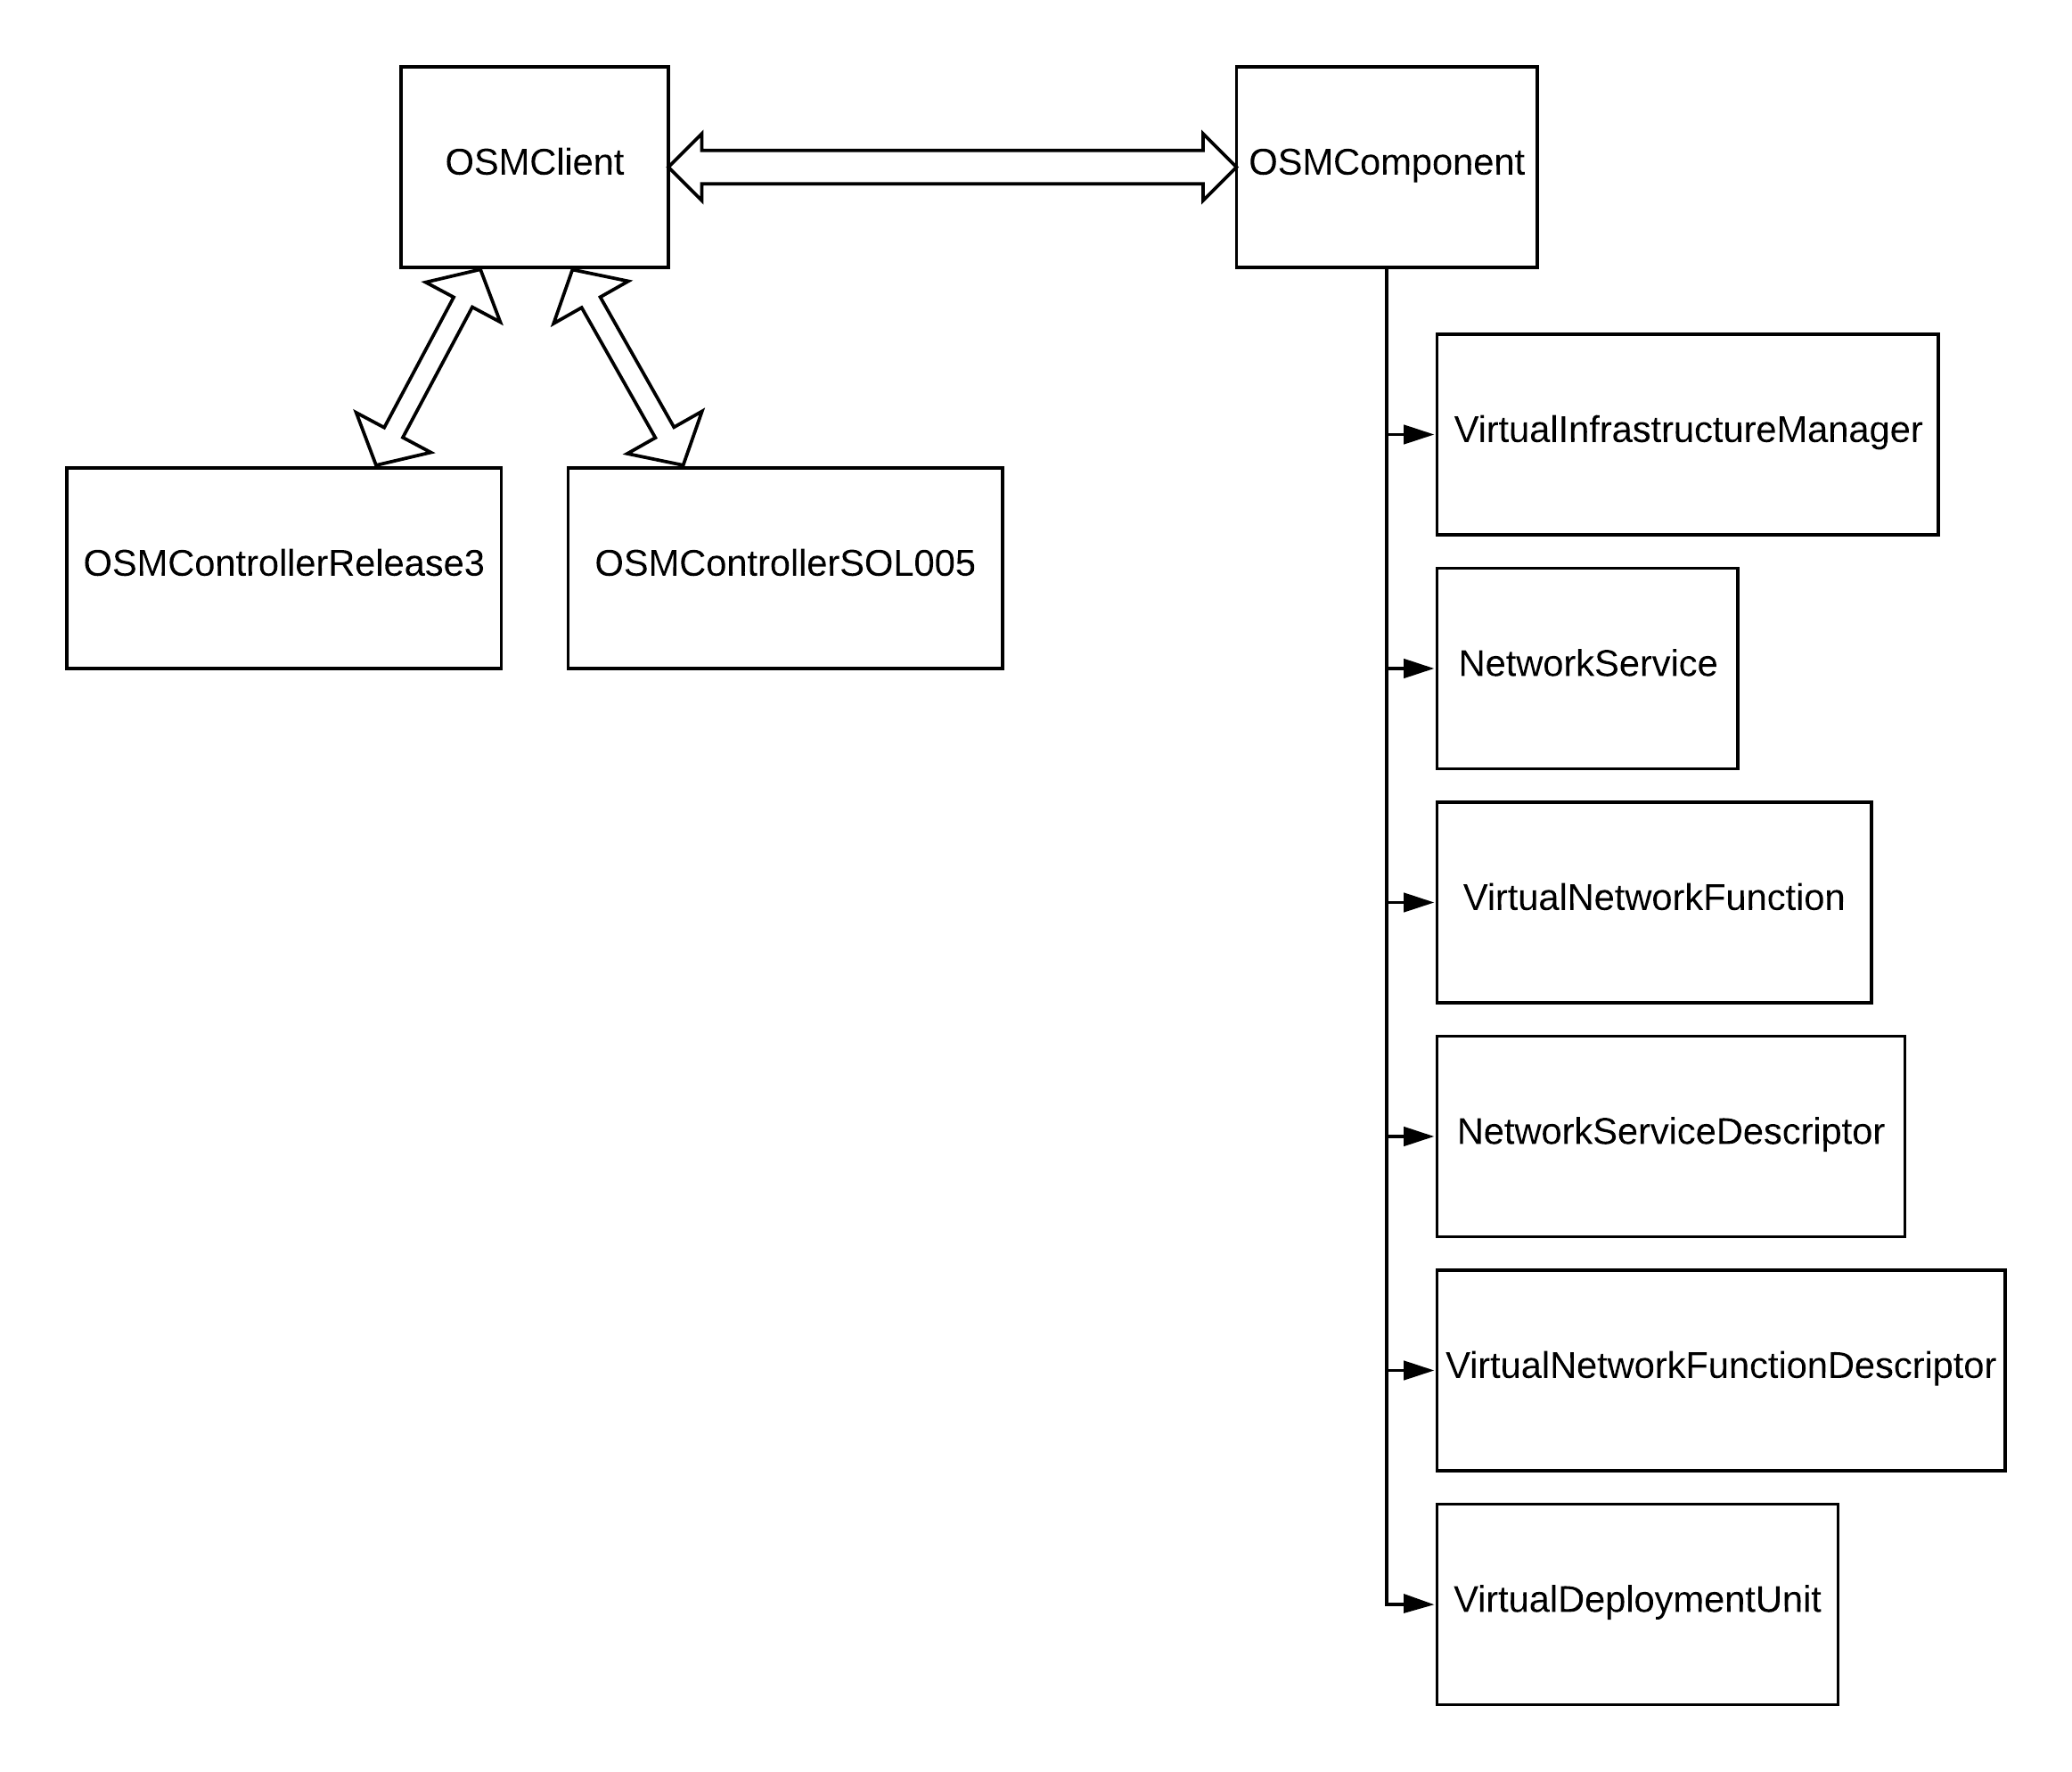
\includegraphics[width=0.7\linewidth]{imagenes/OSMClient}
	\caption{Estructura de clases de J-OSMClient}
	\label{fig:osmclient}
\end{figure}

En la figura \ref{fig:osmclient} se puede ver un esquema detallado de la jerarquía de clases y como dichas clases interaccionan entre sí.


\section{ONOS Client}
\label{sec:onosclient}

\begin{figure}[!ht]
	\centering
	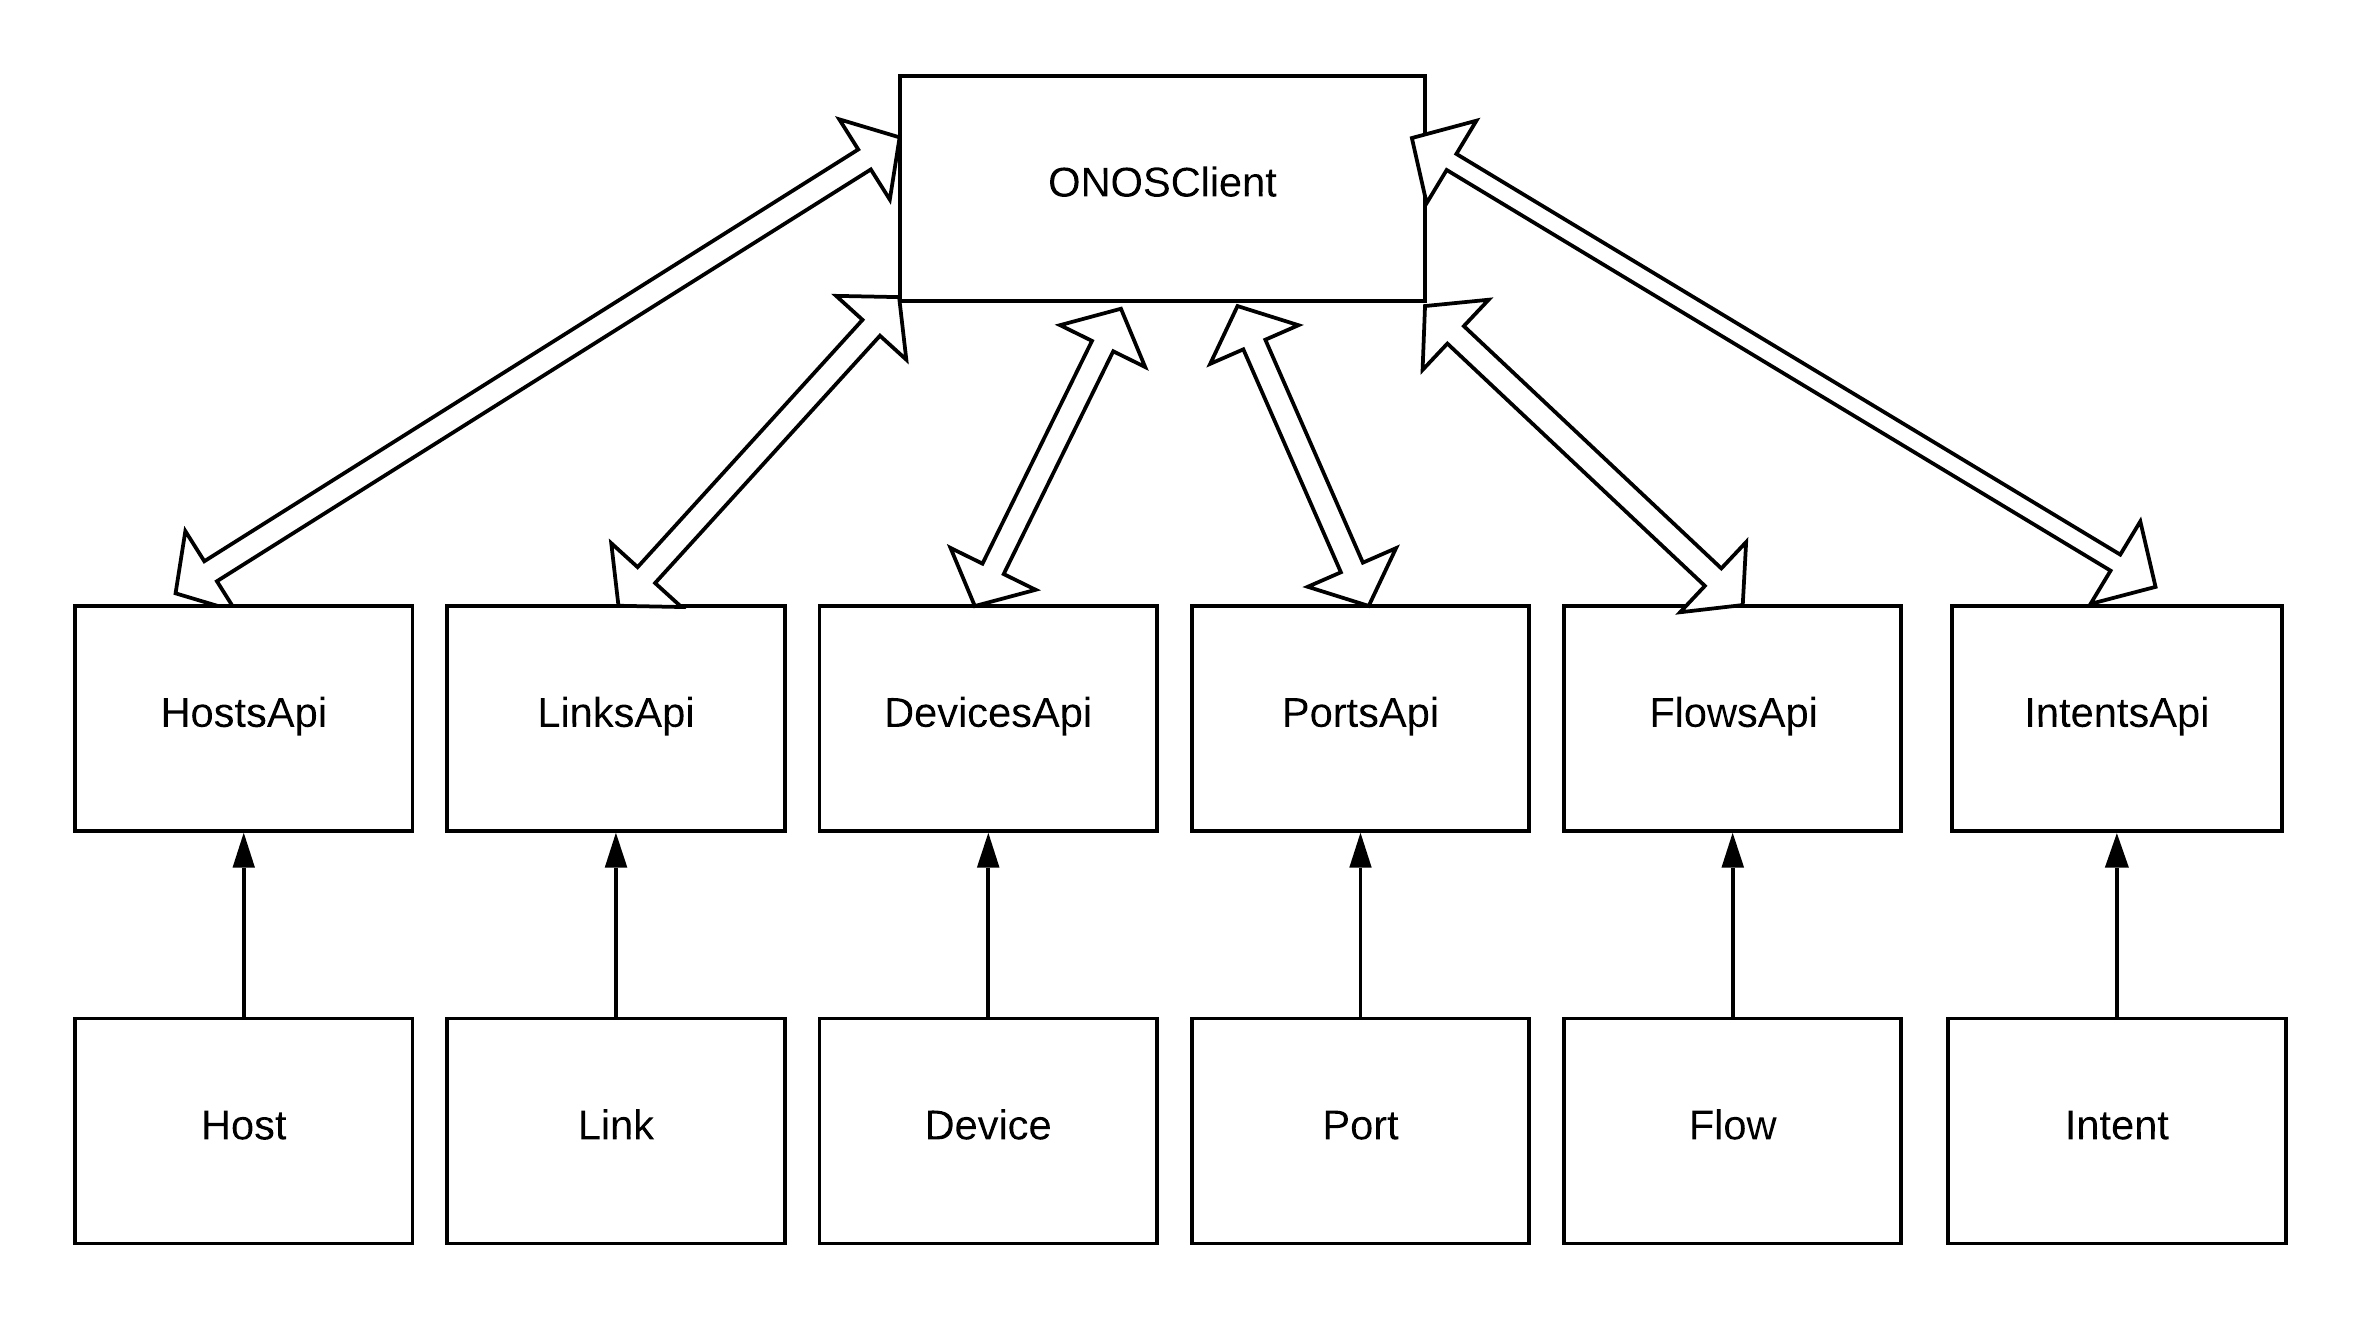
\includegraphics[width=0.7\linewidth]{imagenes/ONOSClient}
	\caption{Estructura de clases de ONOSClient}
	\label{fig:onosclient}
\end{figure}


\section{OpenStack Client}
\label{sec:openstackclient}

\begin{figure}[!ht]
	\centering
	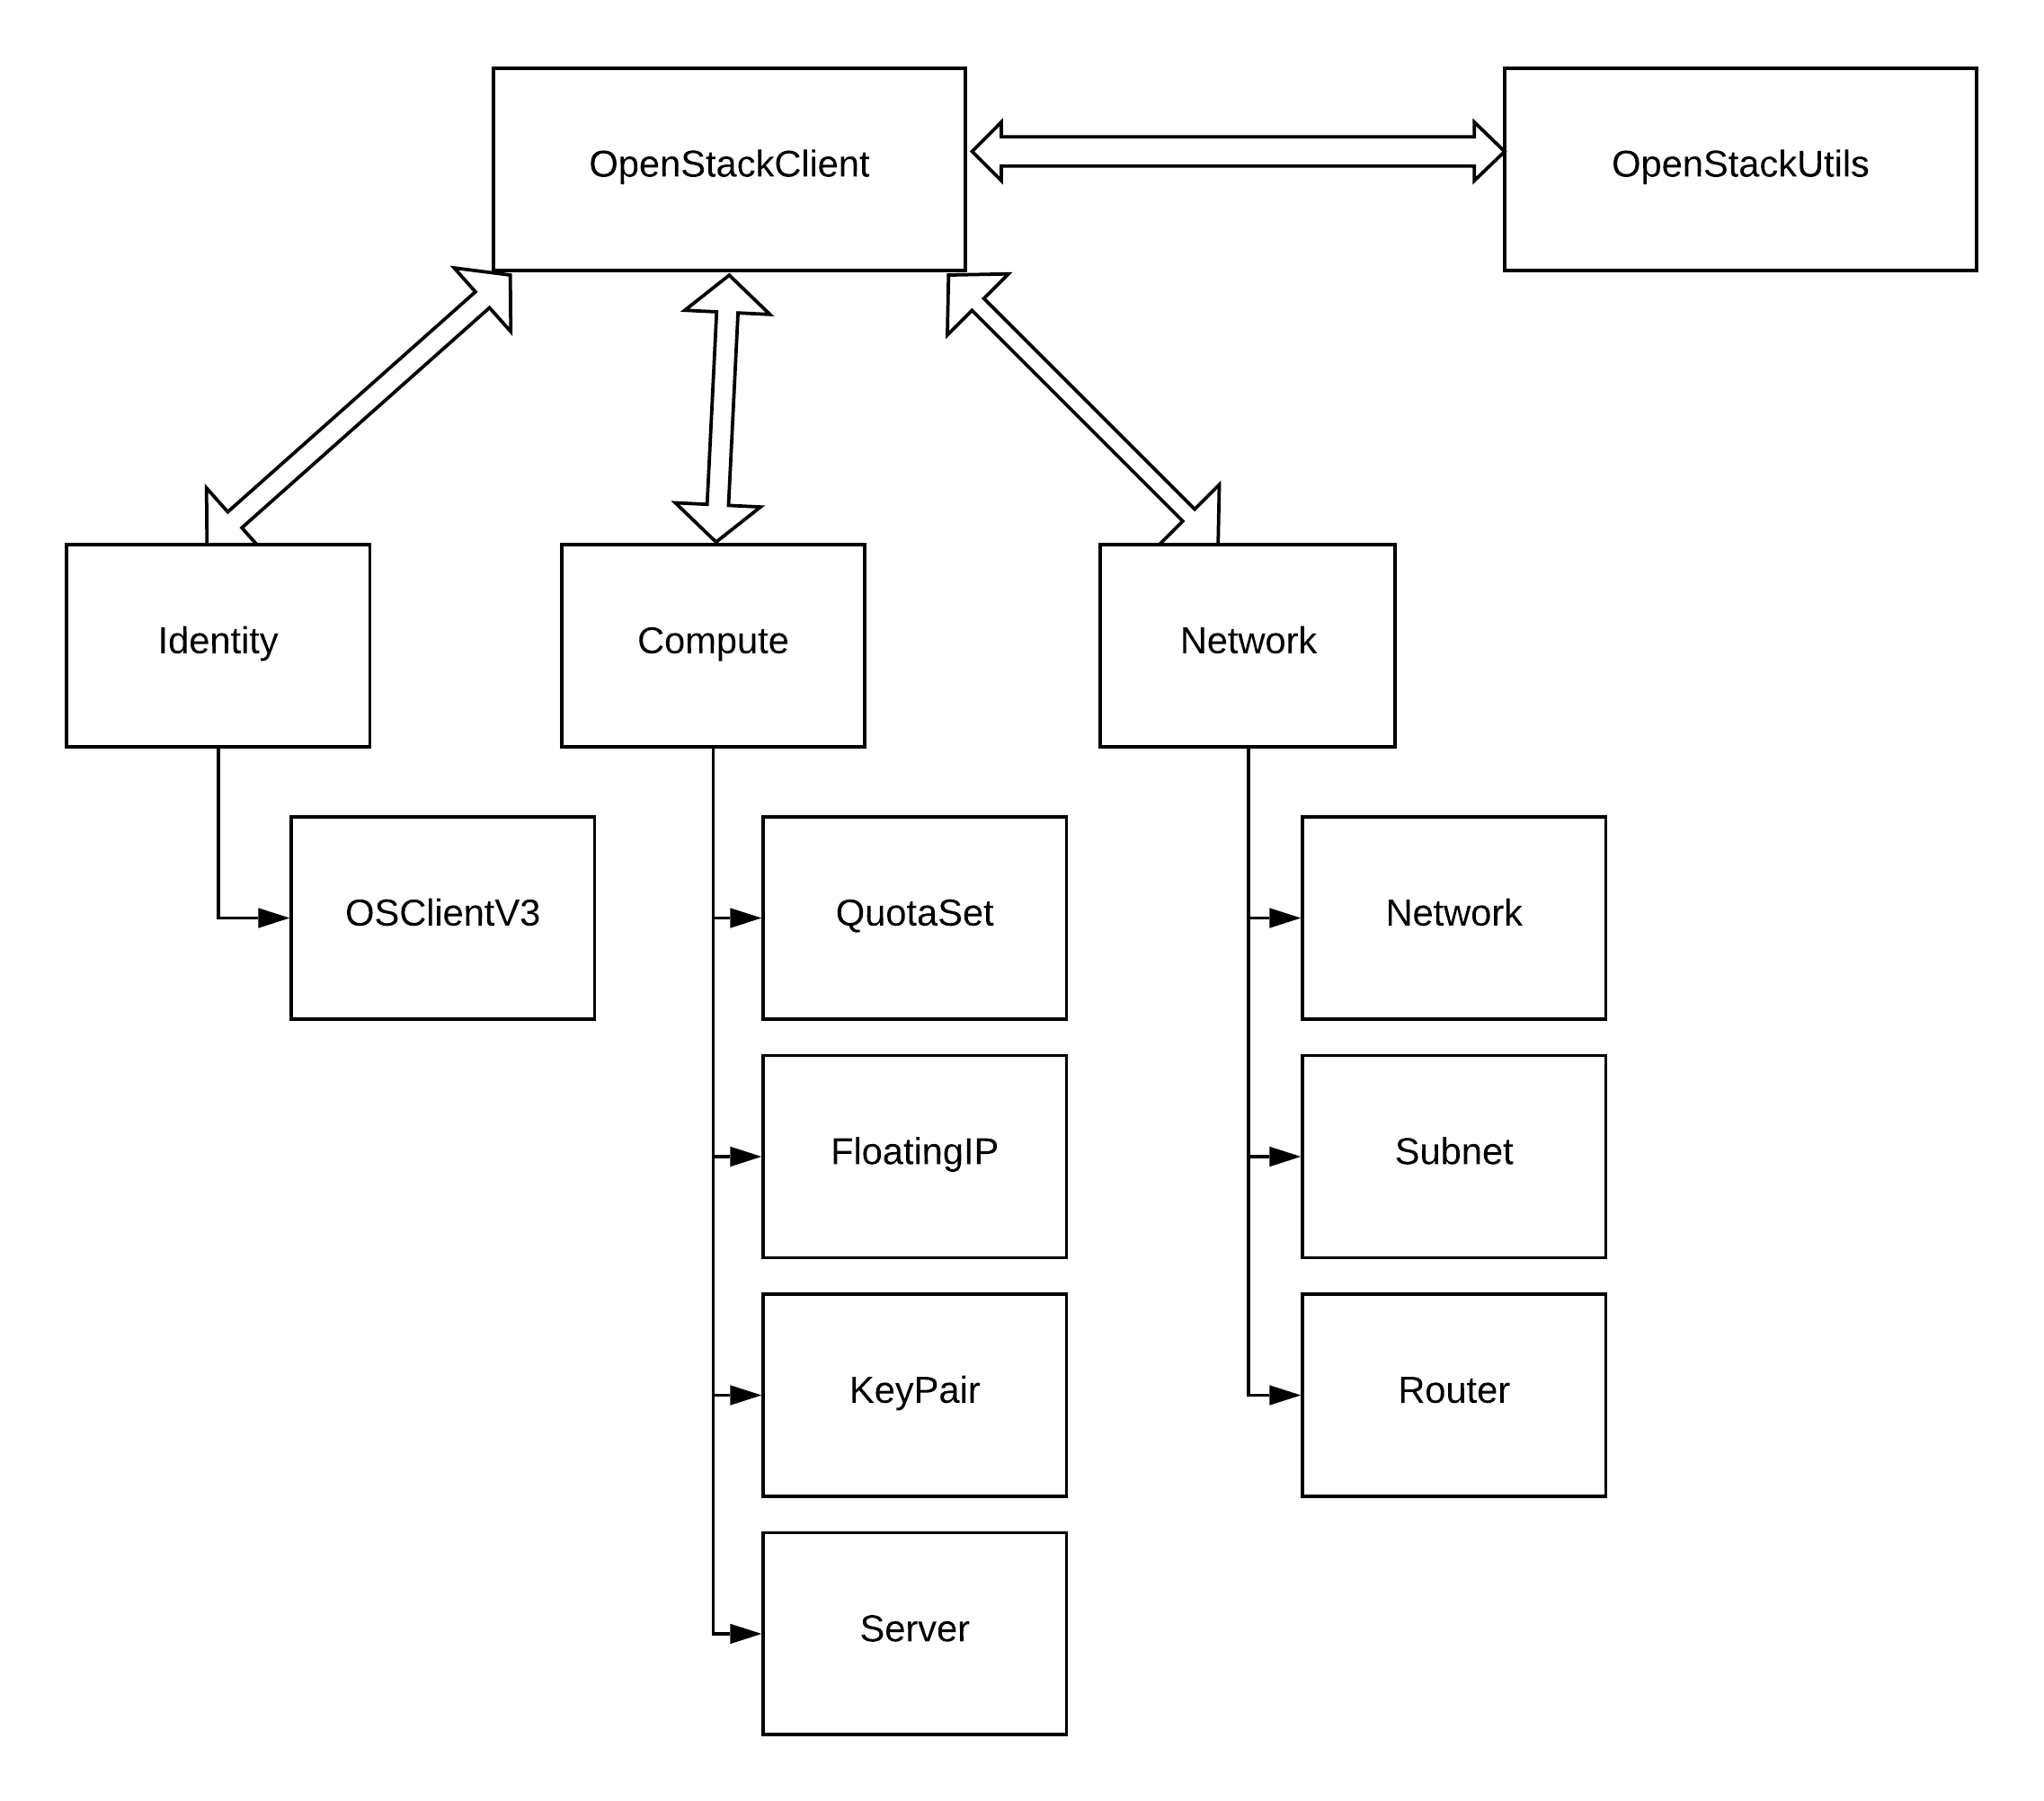
\includegraphics[width=0.7\linewidth]{imagenes/OpenStackClient}
	\caption{Estructura de clases de OpenStackClient}
	\label{fig:openstackclient}
\end{figure}

\section{Net2Plan: NFV Management Plugin}
\label{sec:nfvplugin}

Para llevar a cabo este proyecto, era necesario integrar las APIs mencionadas anteriormente con una herramienta que tenga funcionalidad de planificación de redes. Por ello, se ha desarrollado una extensión de Net2Plan basada en el plugin Network Design.

\begin{figure}[!ht]
	\centering
	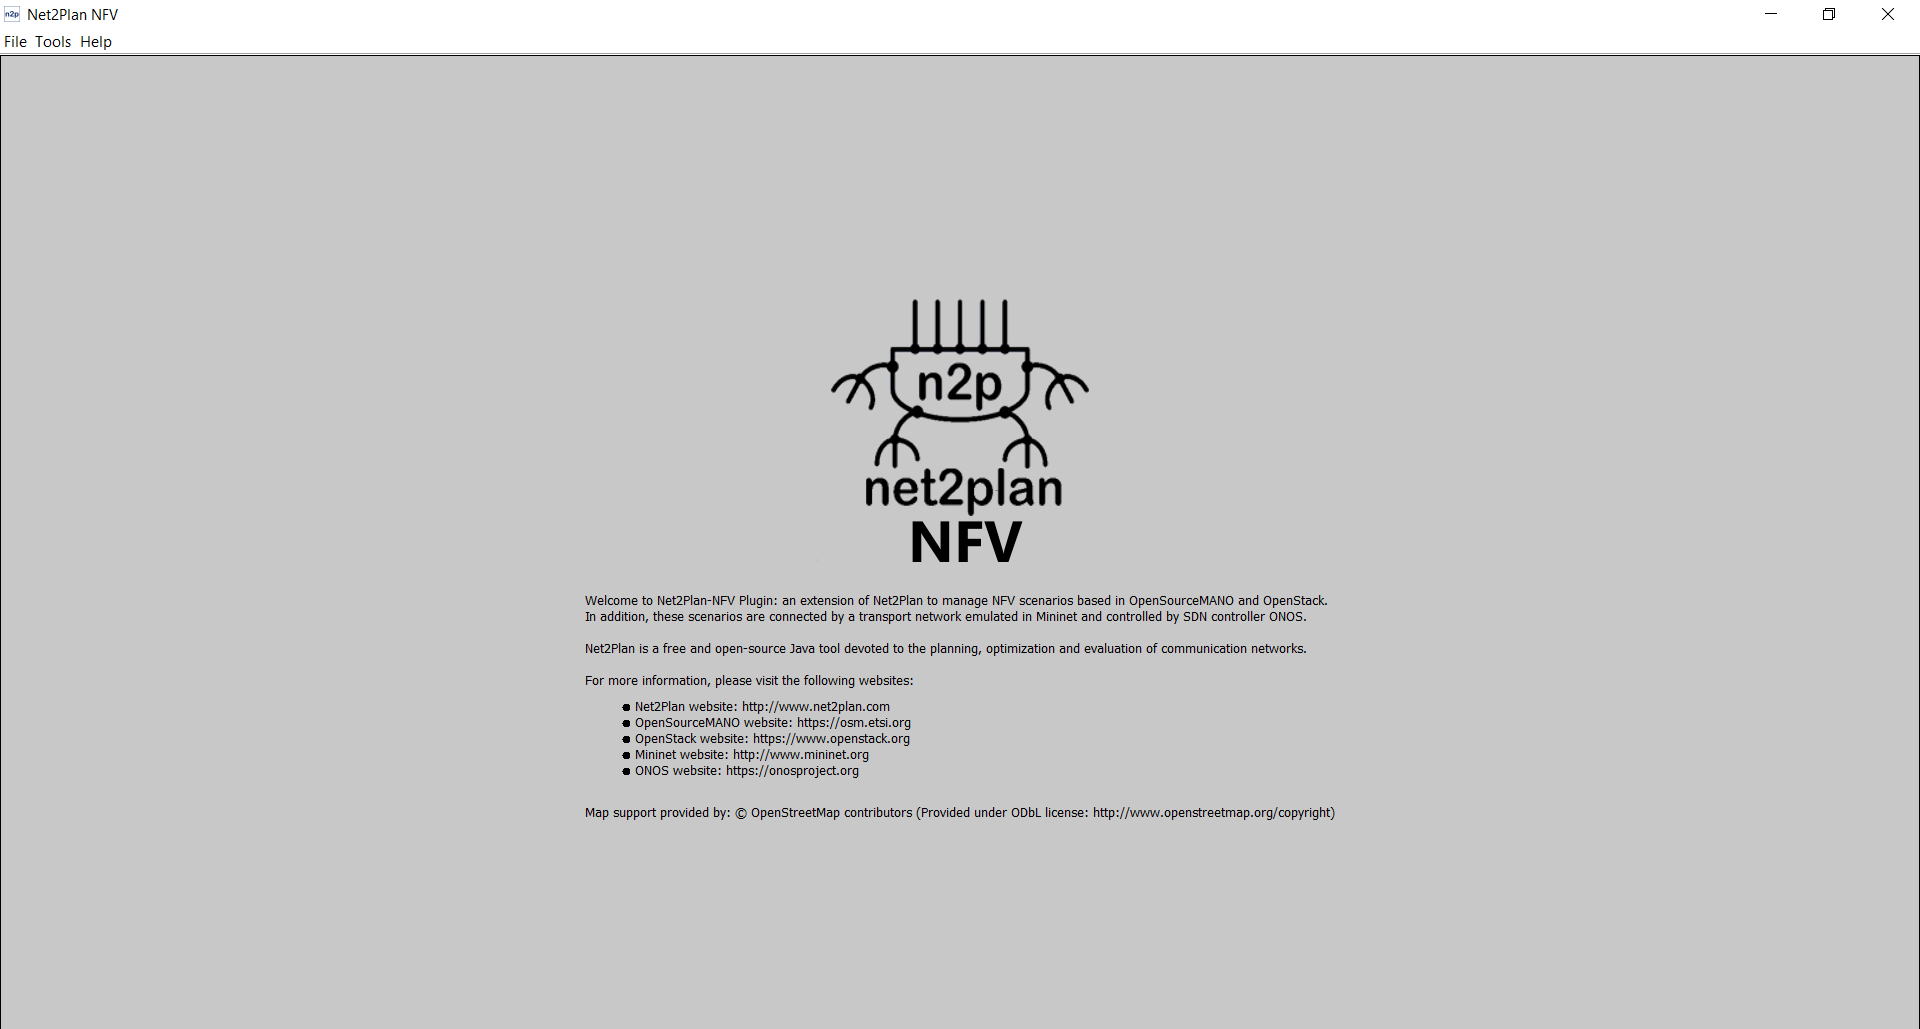
\includegraphics[width=0.8\linewidth]{imagenes/nfvpluginmain}
	\caption{Página de inicio de la extensión Net2Plan-NFV}
	\label{fig:nfvpluginmain}
\end{figure}

\begin{figure}[!ht]
	\centering
	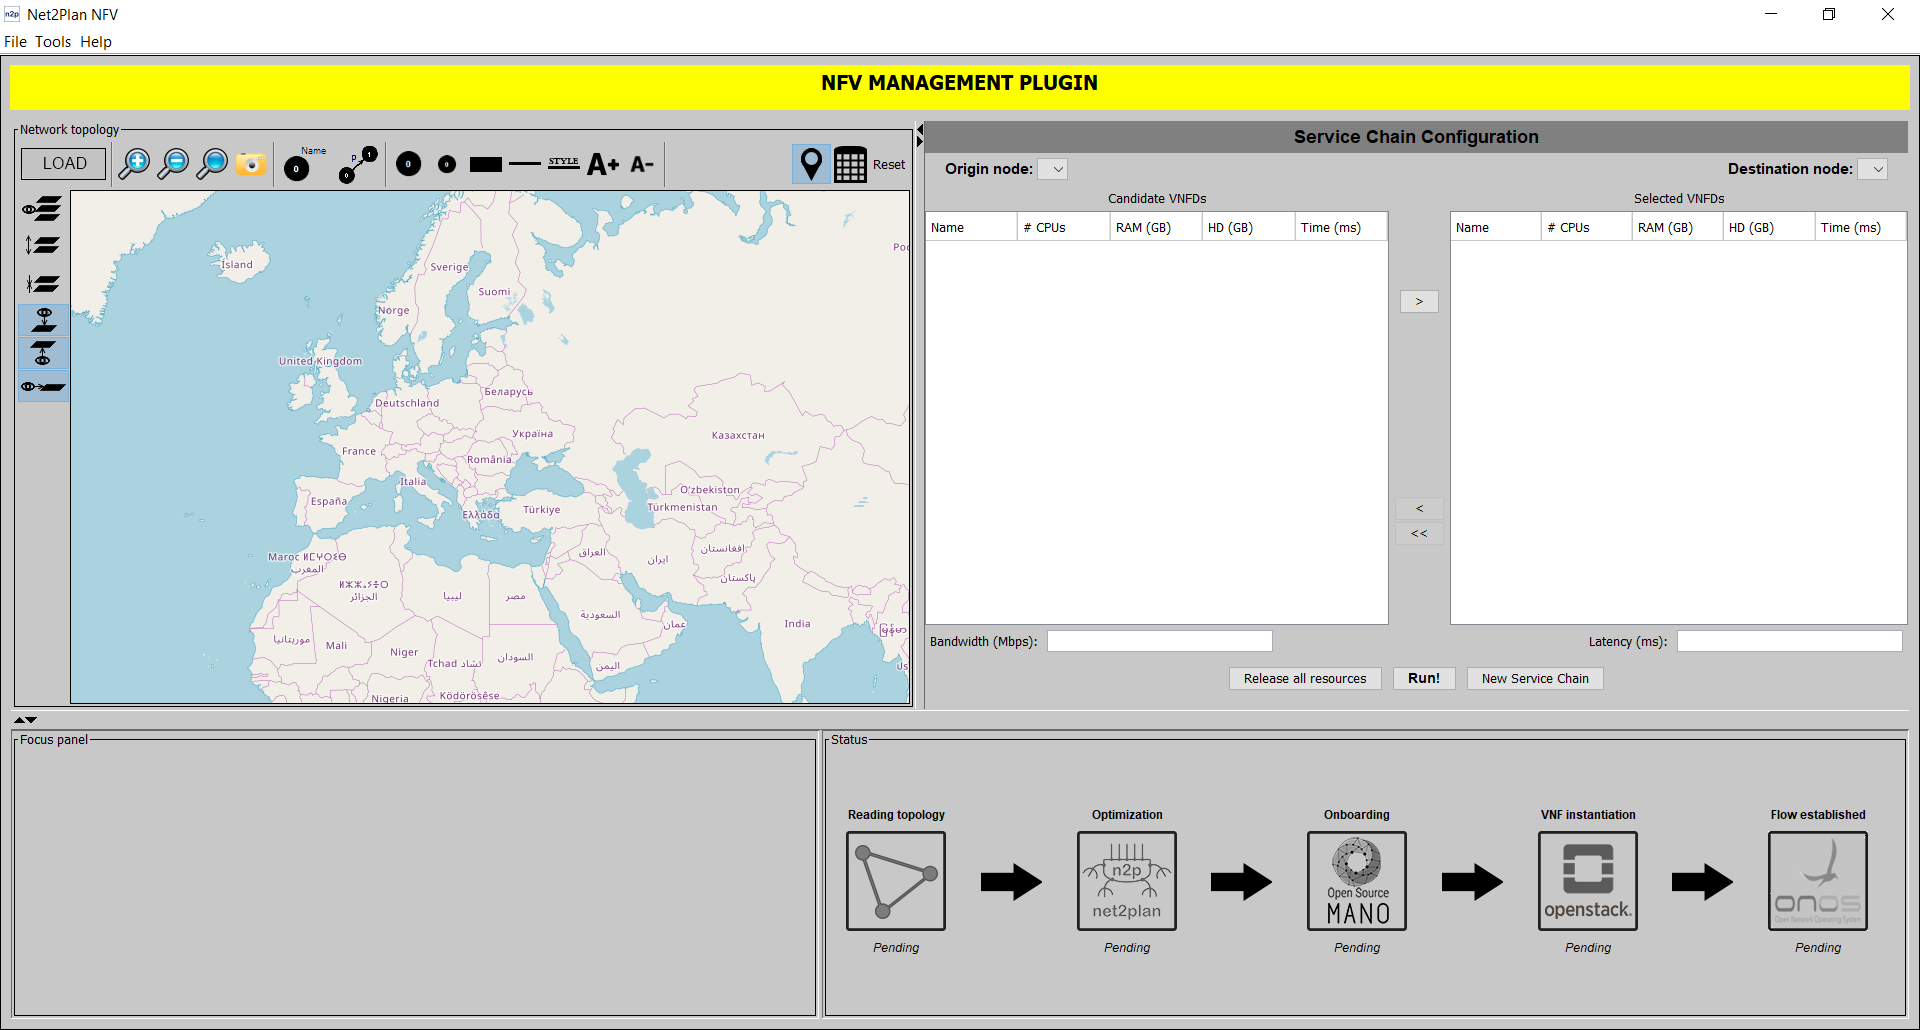
\includegraphics[width=0.8\linewidth]{imagenes/nfvplugin_dashboard}
	\caption{Página de inicio del Plugin NFV-Management}
	\label{fig:nfvplugindash}
\end{figure}






\cleardoublepage % Falta explicar cada api
\chapter{Prueba de concepto}
\label{pruebaconcepto}

En este capítulo se va a hablar de una pequeña prueba de concepto que consiste en un escenario \ac{SDN}-\ac{NFV} donde todas las \acp{API} y herramientas mencionadas en los capítulos \ref{herramientas} y \ref{desarrollo} trabajan conjuntamente en total sintonía.

Inicialmente, se habla sobre el contexto en el que se ha enmarcado la prueba de concepto, haciendo especial referencia al proyecto Metro-Haul.

A continuación, se establece una arquitectura de desarrollo, en la que se define el papel de cada \ac{API} y herramienta, y como interactúan entre sí.

Por último, se realiza una explicación del funcionamiento de la prueba de concepto, así como una vista de los resultados finales.

\section{Contexto}
\label{sec:contexto}

Esta prueba de concepto está enmarcada dentro del proyecto europeo H2020 Metro-Haul\cite{metrohaulbib}. Su principal objetivo es el de diseñar arquitecturas de redes metro que sean accesibles para 5G, anticipándose a los posibles problemas futuros cuando 5G esté totalmente funcional en las redes de telecomunicación.

Estas nuevas arquitecturas aseguran que algunos parámetros de calidad de servicio, como la latencia o el \textit{jitter} sean lo más bajos posibles, así como una total integración de nuevas tecnologías referentes al campo de \ac{ICT}, como son \ac{SDN} y \ac{NFV}.

Para conseguir todos estos objetivos, Metro-Haul busca integrar diferentes herramientas para diseñar nuevas arquitecturas de red. Esta prueba de concepto se planteó como una demostración de como diferentes herramientas podían operar en sintonía para disminuir la latencia al establecer diferentes \textit{Service Chains}, anticipando la llegada del 5G.\cite{demoecocbib}

Dicha demostración tuvo éxito y se publicó en el congreso internacional \ac{ECOC}\cite{ecocbib} en Septiembre de 2018.

\section{Arquitectura}
\label{sec:arquitectura}

El principal objetivo de la prueba de concepto es el de integrar todas las \acp{API} y herramientas mencionadas anteriormente para conseguir satisfacer diferentes \textit{Service Chains} con restricciones de latencia y ancho de banda. Además, se busca demostrar como todas las herramientas \textit{open-source} que componen dicha prueba de concepto trabajan en sintonía para crear un escenario \ac{SDN}-\ac{NFV} heterogéneo.

Para conseguir los objetivos mencionados anteriormente, se ha diseñado una arquitectura específica para poder llevar a cabo la prueba de concepto, donde cada uno de los elementos realiza una tarea en concreto.

\begin{figure}[!ht]
	\centering
	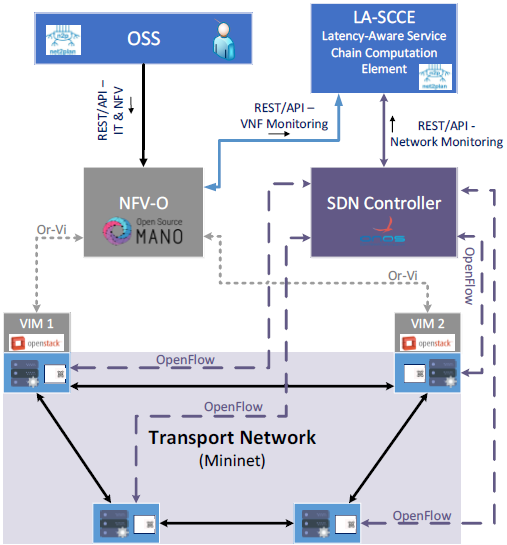
\includegraphics[width=0.7\linewidth]{imagenes/esquema_demo}
	\caption{Arquitectura de la Prueba de Concepto. Fuente:\cite{demoecocbib}}
	\label{fig:esquemademo}
\end{figure}

En la figura \ref{fig:esquemademo} se puede observar un esquema de la arquitectura, en el que se incluyen todos los elementos que la componen, y hace más fácil de entender como interactúan entre sí los componentes.

A continuación vemos una explicación de cada uno de los elementos que componen la prueba de concepto y que componente lleva a cabo esa acción:

\begin{itemize}
	\item \textbf{\ac{OSS}:} representa el papel de un operador que despliega un servicio gracias a una aplicación. El operador es emulado mediante la \ac{GUI} de Net2Plan, más concretamente por su plugin de \textit{NFV Management} (ver \ref{sec:nfvplugin}).
	
	\item \textbf{\ac{NFV-O}:} representa el papel de una aplicación que se encarga de gestionar la infraestructura de virtualización necesaria para instanciar diferentes máquinas virtuales. \ac{OSM} (ver \ref{sec:osm}) es el encargado de dicha función.
	
	\item \textbf{\acp{VIM}:} son los encargados de instanciar y alojar las diferentes máquinas virtuales pertenecientes a los VNF. OpenStack (ver \ref{sec:openstack}) es quien realiza este papel.
	
	\item \textbf{Red de Transporte:} la red de transporte es emulada mediante Mininet (ver \ref{sec:mininet}) para establecer flujos de paquetes entre las diferentes \acp{VNF} de una \textit{Service Chain}. La red se define mediante un script en Python (ver anexo \ref{sec:scriptmininet}).
	
	\item \textbf{Controlador \ac{SDN}:} la red de transporte es controlada por una instancia de \ac{ONOS} (ver \ref{sec:onos}) mediante el envio de paquetes Openflow (ver \ref{subsec:openflow}) a los diferentes switches de la red.
	
	\item \textbf{\ac{LA-SCCE}:} Se encarga de decidir el camino a seguir para atravesar una secuencia de \acp{VNF} que cumpla con los requisitos de latencia máxima. Este papel lo representa un algoritmo programado en Net2Plan para resolver de forma conjunta tanto el camino como el emplazamiento de las \acp{VNF} óptimos.
\end{itemize}


\section{Funcionamiento}
\label{sec:funcprueba}

Para llevar a cabo la prueba de concepto, la arquitectura explicada en la sección anterior se ha traducido en un \textit{testbed} para poder llevarla a cabo, como se puede apreciar en la figura \ref{fig:poctestbed}.

\begin{figure}[!ht]
	\centering
	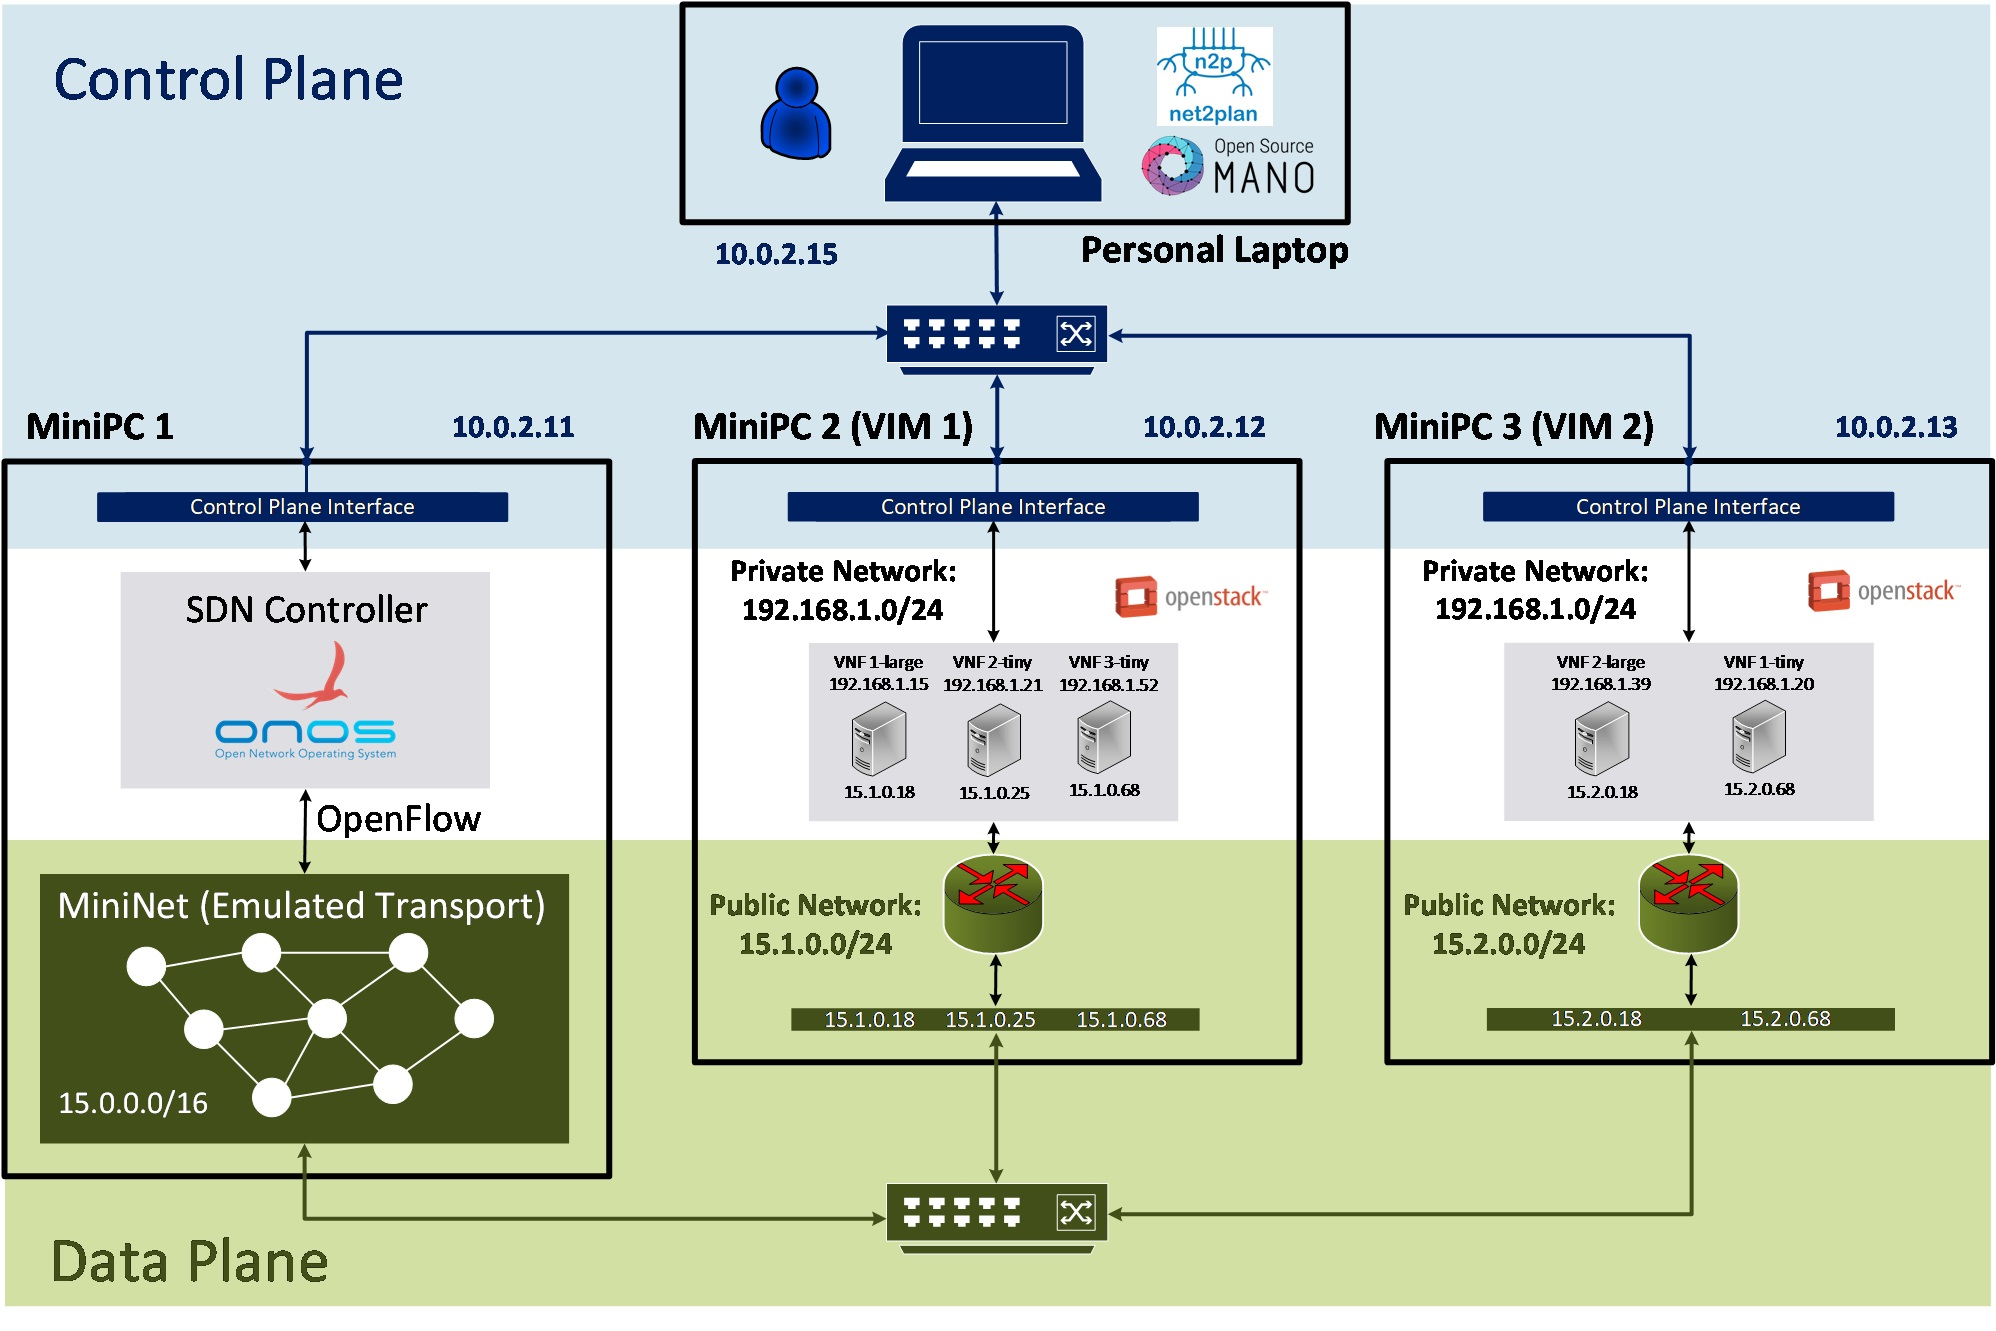
\includegraphics[width=0.9\linewidth]{imagenes/PoC_testbed}
	\caption{\textit{Testbed} para la Prueba de Concepto. Fuente:\cite{demoecocbib}}
	\label{fig:poctestbed}
\end{figure}

El \textit{testbed} considerado se compone de cuatro \acp{PC} y dos \textit{switches}, uno para el plano de control y otro para el plano de datos:

\begin{itemize}
	\item \textbf{Mini\ac{PC}1:} Este \ac{PC} se encarga de alojar una instancia del controlador \ac{SDN} \ac{ONOS} y de emular la red de transporte gracias a Mininet.
	
	\item \textbf{Mini\ac{PC}2:} En este \ac{PC} se encuentra corriendo una instancia de OpenStack, que actúa como \ac{VIM} 1.
	
	\item \textbf{Mini\ac{PC}3:} En este \ac{PC} se encuentra corriendo una instancia de OpenStack, que actúa como \ac{VIM} 2.
	
	\item \textbf{\textit{Personal Laptop}:} Este dispositivo actúa como entidad central del \textit{testbed}. En él se encuentra corriendo una instancia de \ac{OSM} y el plugin \textit{NFV Management} de Net2Plan.
\end{itemize}


Una vez explicado el \textit{testbed}, se explican los diferentes pasos que se realizan para llevar a cabo la prueba de concepto y que \acp{API} intervienen en cada uno de ellos:

\begin{itemize}
	
	\item \textbf{Paso 1.} Una vez que \ac{ONOS}, \ac{OSM} y los \acp{VIM} estan listos y corriendo, se arranca el plugin de Net2Plan para comenzar con la demostración.
	
	\begin{figure}[!ht]
		\centering
		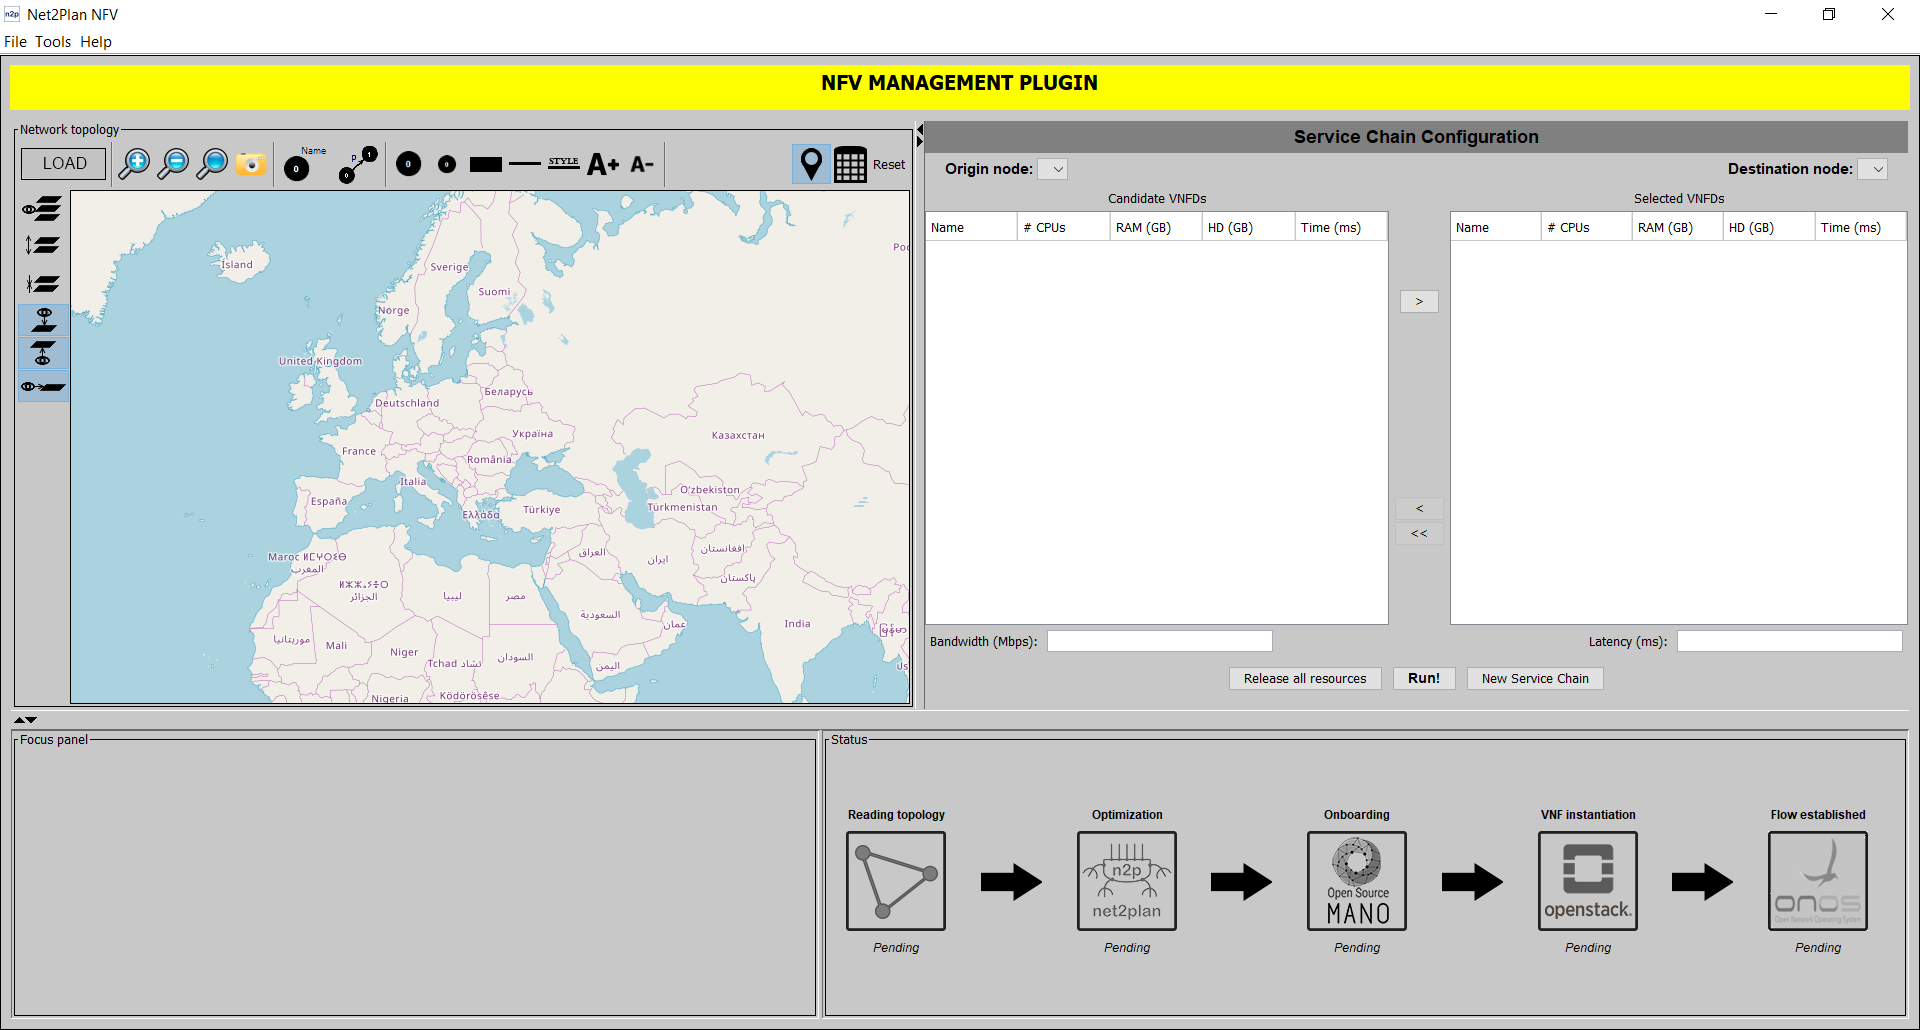
\includegraphics[width=0.9\linewidth]{imagenes/nfvplugin_dashboard}
		\caption{Interfaz gráfica del Plugin al inicio}
		\label{fig:nfvproof_inicio}
	\end{figure}
	
	\item \textbf{Paso 2.} Haciendo click en el botón LOAD, Net2Plan recibe la información referente a la red de transporte de \ac{ONOS} haciendo uso de J-ONOSClient, la información sobre los posibles \acp{VNF} a instanciar en \ac{OSM} haciendo uso de J-OSMClient y la información sobre cada \ac{VIM} de OpenStack haciendo uso de J-OpenStackClient.
	
	\item \textbf{Paso 3.} El usuario define la \textit{Service Chain} que se quiere satisfacer (nodo origen, nodo destino, secuencia ordenada de VNFs a atravesar, latencia máxima y ancho de banda) a través de la interfaz gráfica del Plugin.
	
	\clearpage
	
	\item \textbf{Paso 4.} Net2Plan recibe la información introducida por el usuario y la transfiere al \ac{LA-SCCE} para que ejecute el algoritmo que devolverá como resultado una ruta de enlaces para la \textit{Service Chain} y el \ac{VIM} donde cada \ac{VNF} debe ser instanciado.
	
		\begin{figure}[!ht]
		\centering
		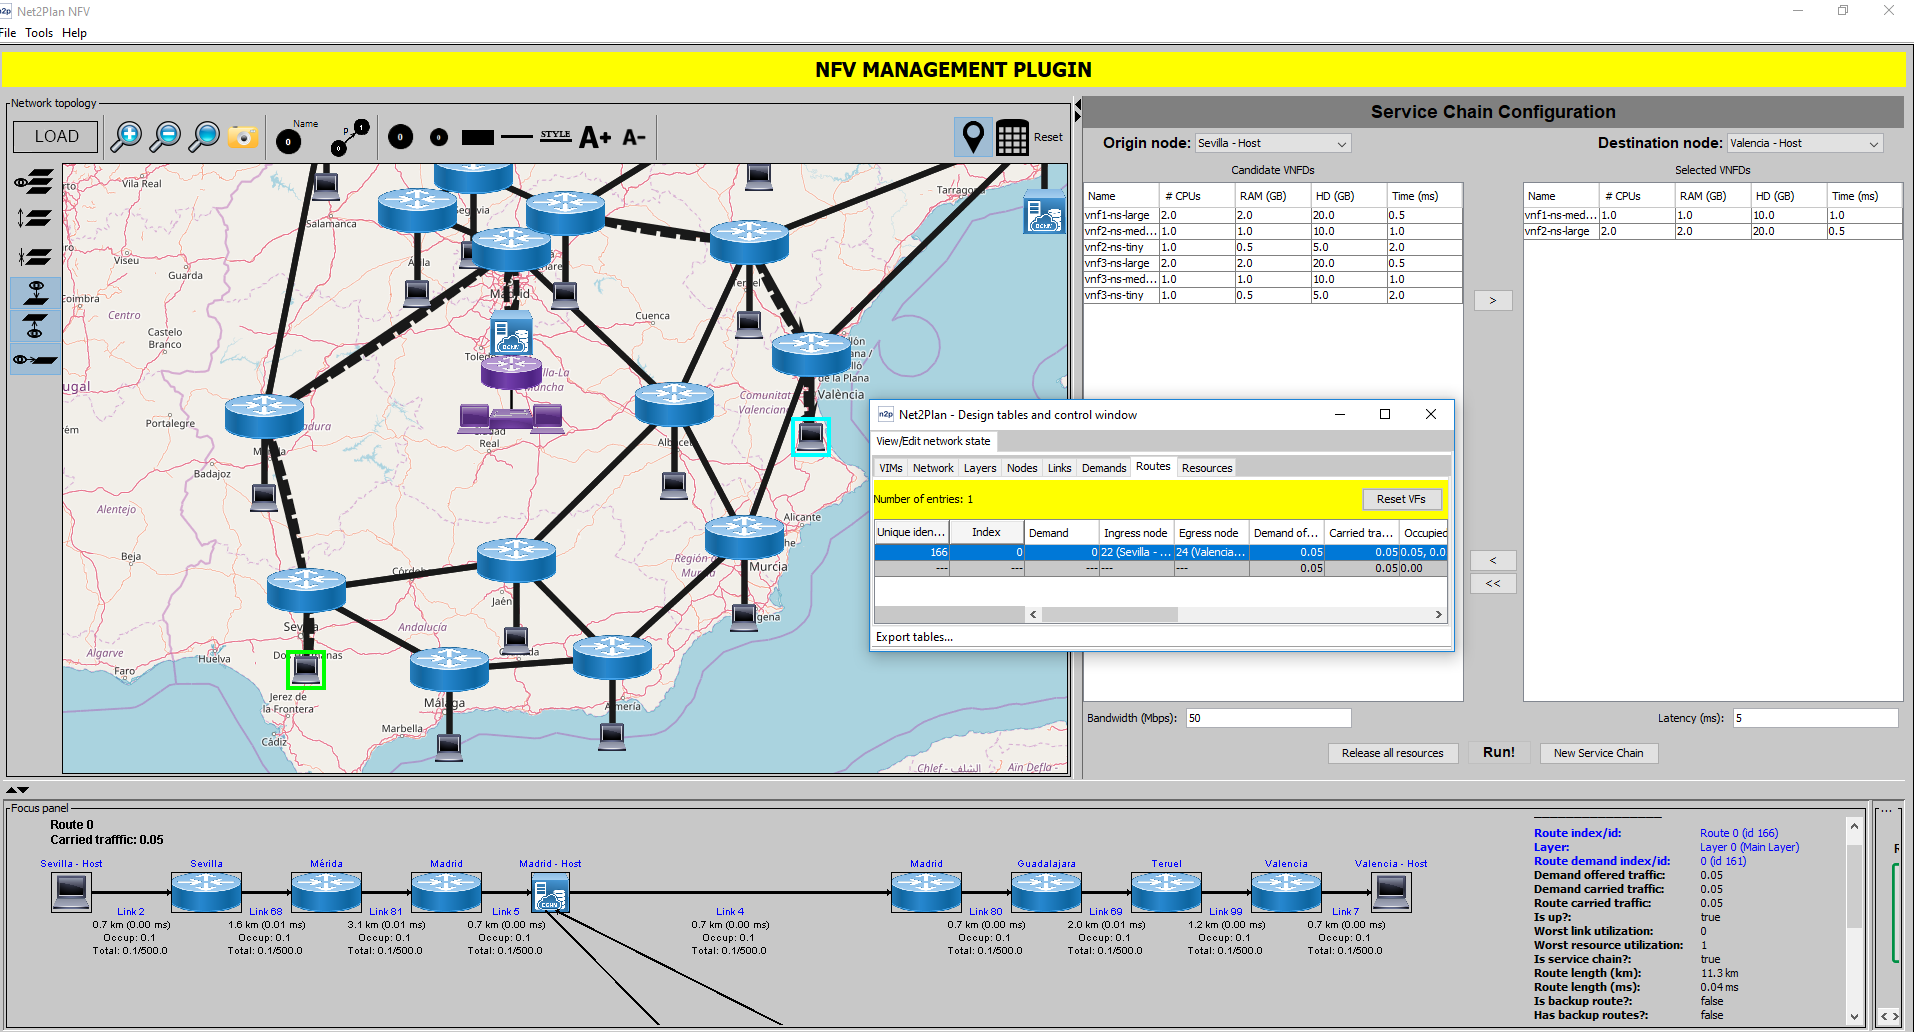
\includegraphics[width=0.9\linewidth]{imagenes/nfv_service_chain}
		\caption{Interfaz gráfica del Plugin con la ruta establecida}
		\label{fig:nfvservicechain}
	\end{figure}

	En la figura \ref{fig:nfvservicechain} se apreciar la ruta obtenida por el algoritmo en la \ac{GUI} de Net2Plan.
	
	\item \textbf{Paso 5.} Net2Plan envía la orden a \ac{OSM} haciendo uso de J-OSMClient de instanciar los distintos \acp{VNF} en los \acp{VIM} que el \ac{LA-SCCE} obtuvo como óptimos.
	
	\begin{figure}[!ht]
		\centering
		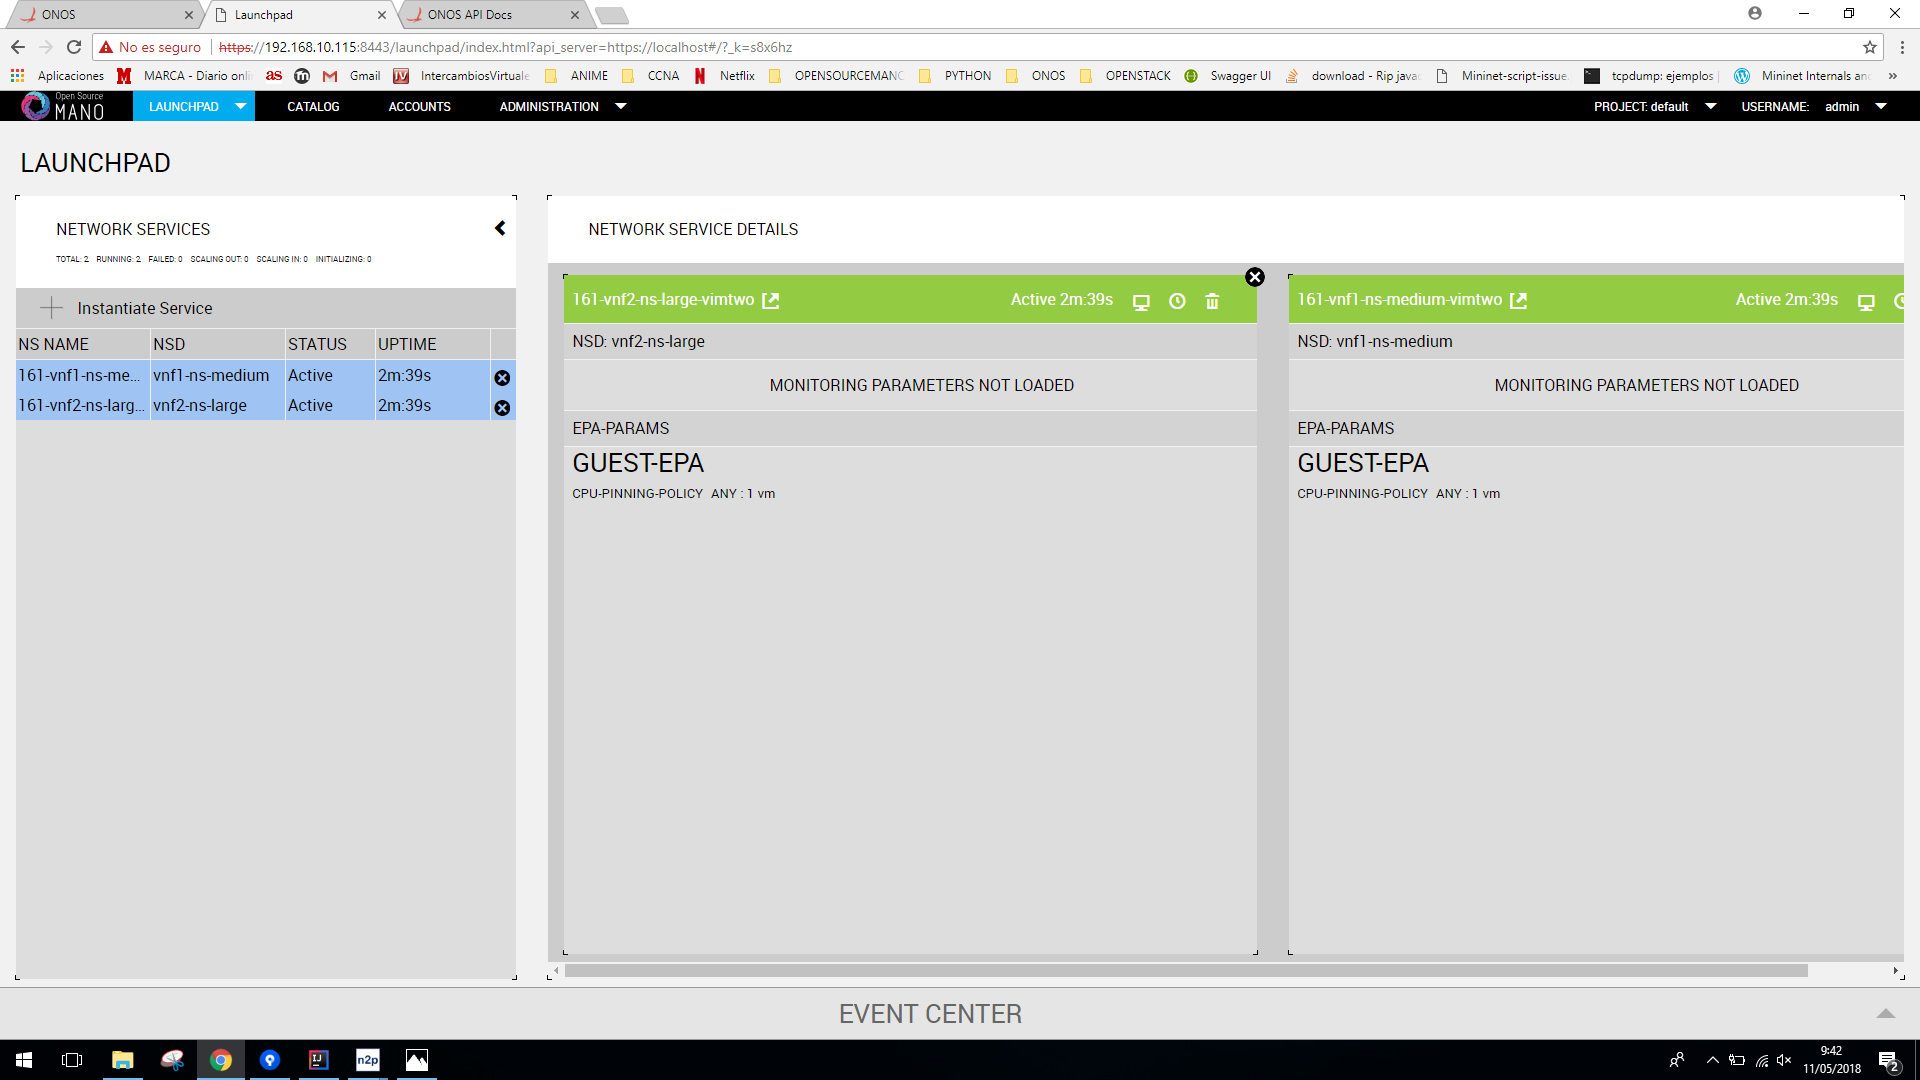
\includegraphics[width=0.9\linewidth]{imagenes/osm_vnfs}
		\caption{Interfaz gráfica de \ac{OSM} con los \acp{VNF} instanciados}
		\label{fig:osmvnfs}
	\end{figure}
	
	En la figura \ref{fig:osmvnfs} se puede apreciar como \ac{OSM} ha instanciados los \acp{VNF} en los \acp{VIM} según los cálculos del algoritmo.
	
	\item \textbf{Paso 6.} \ac{OSM} envia órdenes a los diferentes \acp{VIM} para que alojen las diferentes máquinas virtuales correspondientes a los \acp{VNF}. La comunicacion entre \ac{OSM} y OpenStack es transparente al usuario.
	
	\item \textbf{Paso 7.} Net2Plan envía la orden a \ac{ONOS}, haciendo uso de J-ONOSClient, con diferentes reglas de flujo para establecer en los diferentes \textit{switches} de la red de transporte, todo según la ruta óptima obtenida por el \ac{LA-SCCE}.
	
	\begin{figure}[!ht]
		\centering
		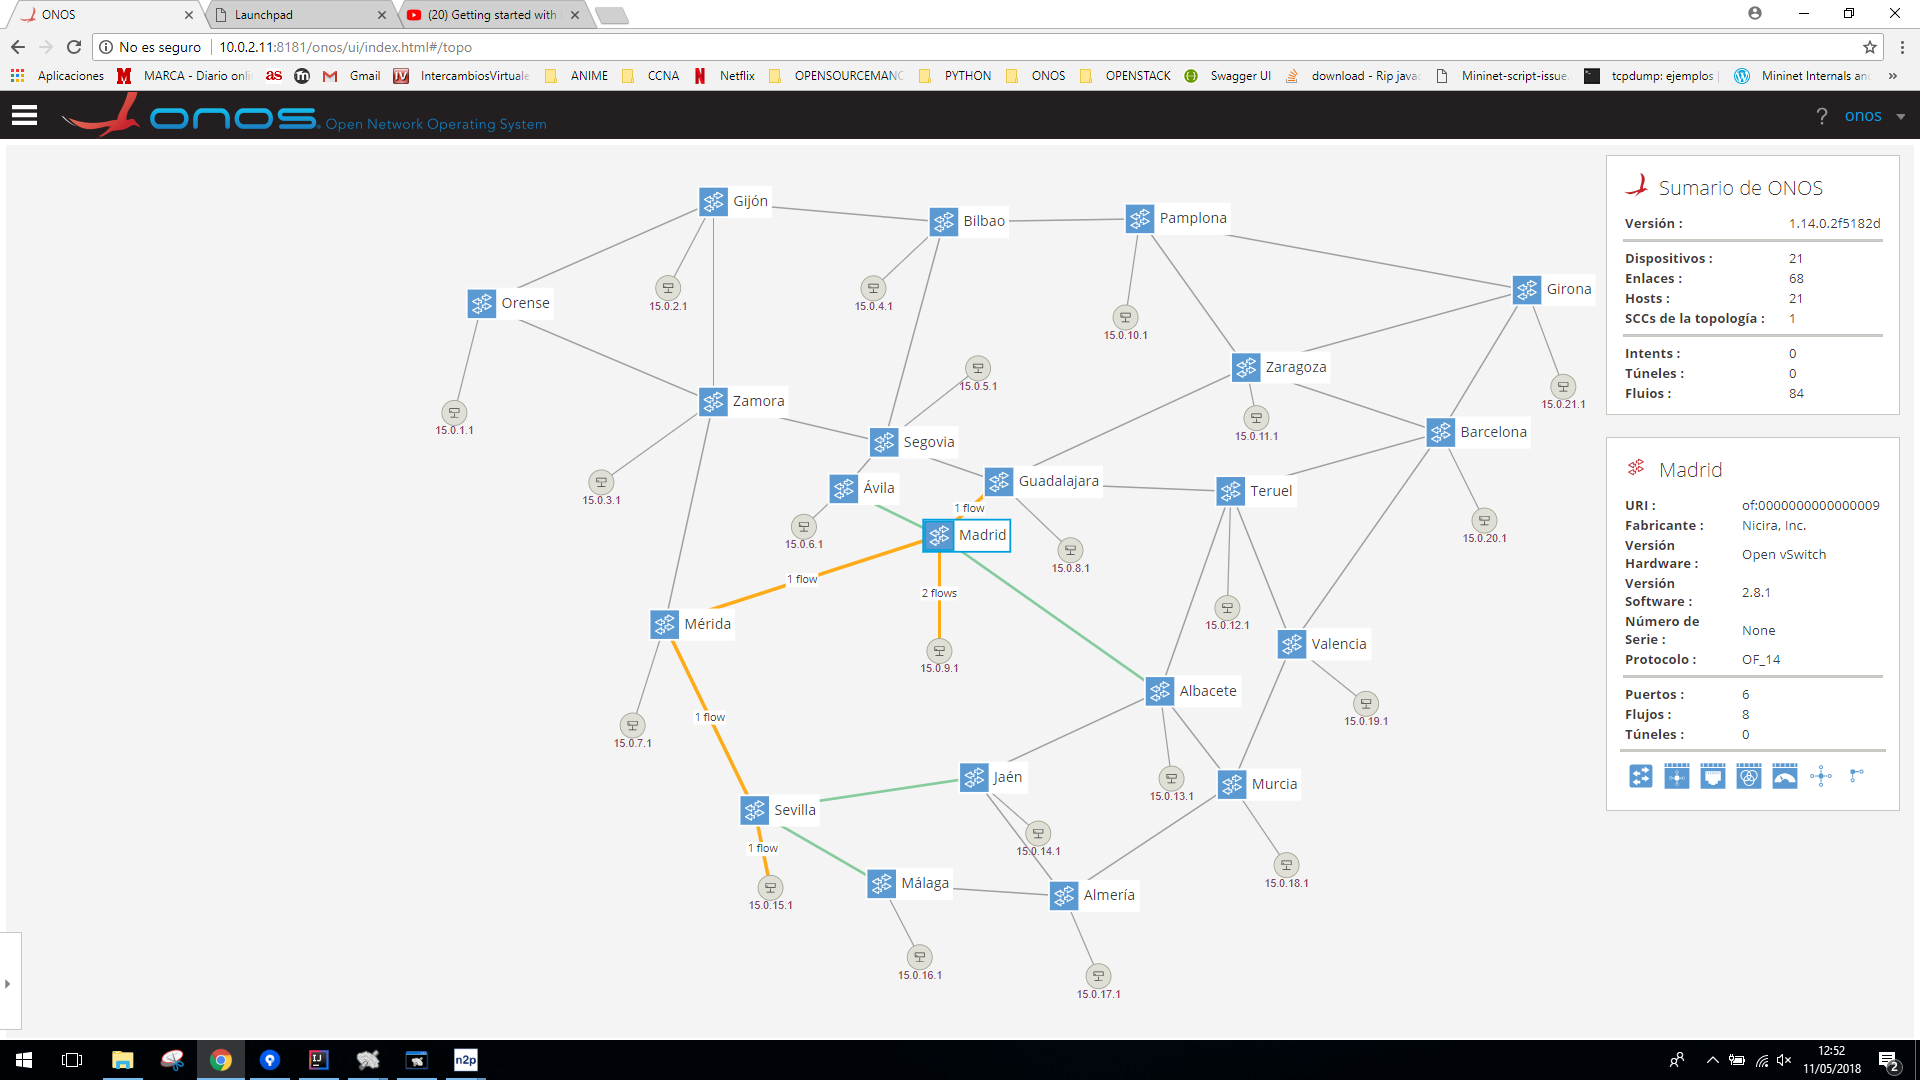
\includegraphics[width=0.9\linewidth]{imagenes/topo_onos}
		\caption{Interfaz gráfica de \ac{ONOS} con las reglas de flujo establecidas}
		\label{fig:topo_onos}
	\end{figure}

	En la figura \ref{fig:topo_onos} se puede apreciar como la ruta calculada en Net2Plan se traslada a \ac{ONOS}.

	\item \textbf{Paso 8.} Una vez establecidas las reglas de flujo en los diferentes \textit{switches} mediante OpenFlow, se realiza una prueba de conexión para asegurar que la \textit{Service Chain} está establecida y se satisface correctamente.
	
	\begin{figure}[!ht]
		\centering
		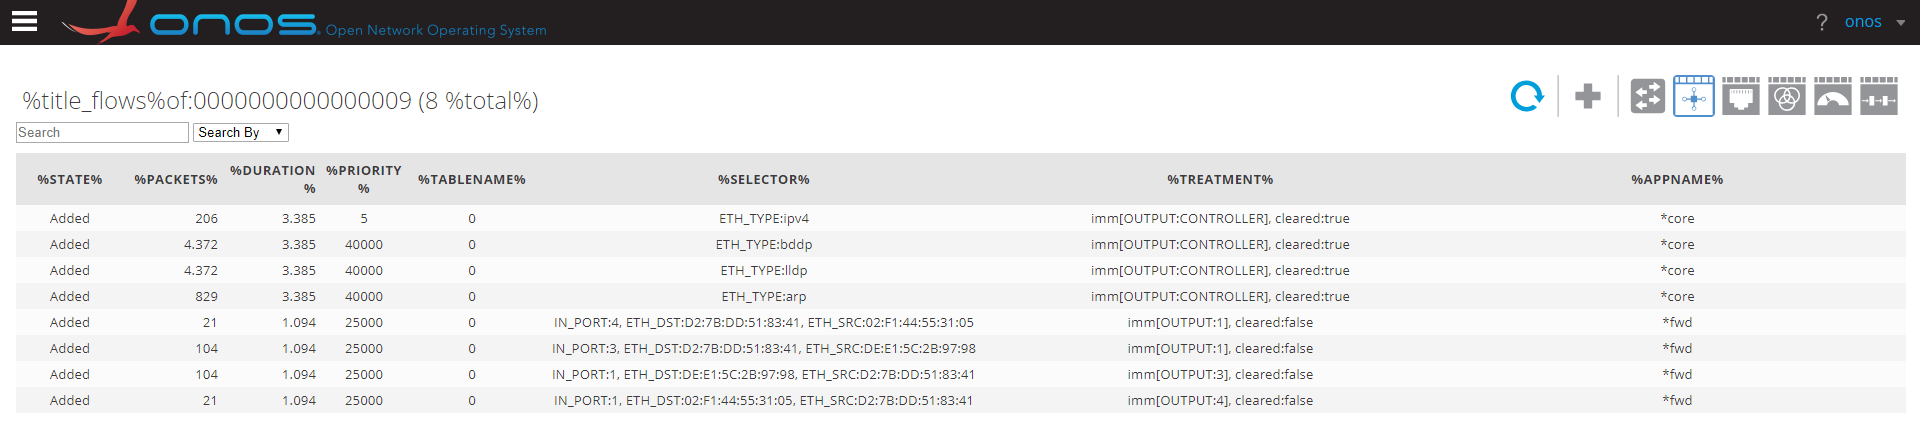
\includegraphics[width=0.9\linewidth]{imagenes/onos_flowrules}
		\caption{Prueba de conectividad en la \ac{GUI} de \ac{ONOS}}
		\label{fig:onosflowrules}
	\end{figure}

	En la figura \ref{fig:onosflowrules} se puede apreciar la instalación de reglas de flujo en \ac{ONOS} que sirven para satisfacer la \textit{Service Chain}.

\end{itemize}

Tras llevar a cabo la prueba de concepto, hay que mencionar los resultados obtenidos. Una vez instanciados los \acp{VNF} correspondientes a la \textit{Service Chain} y habiendo instalado las reglas de flujo correspondientes a la ruta óptima obtenida en los \textit{switches}, se realizan una prueba de conexión enviando un ping entre el origen y el destino. 

En la figuras \ref{fig:nfvservicechain} y \ref{fig:topo_onos} se puede observar como la ruta es la misma en ambos casos (en el plugin de Net2Plan y en \ac{ONOS}), y en la figura \ref{fig:onosflowrules} como las reglas de flujo aplicadas indican que han procesado un paquete, que corresponde al ping realizado anteriormente para validad la conectividad.

 % Terminado (A falta de ver más fotos para completar la explicación)
\chapter{Conclusiones}
\label{conclusiones}

El objetivo inicialmente propuesto fue el desarrollo de diferentes \acp{API} para comunicar diferentes herramientas \textit{open-source} entre sí para poder diseñar un escenario \ac{SDN}-\ac{NFV} heterogéneo.

Una vez establecidos los objetivos, se comenzó con el desarrollo de J-OSMClient, J-ONOSClient y J-OpenStackClient para poder establecer la comunicación con \ac{OSM}, \ac{ONOS} y OpenStack, gracias a las \acp{API} \ac{REST} que exportan cada uno de ellos.

Una vez los clientes estuvieron totalmente funcionales, se comenzó con el desarrollo del plugin \textit{NFV Management}, para convertir a Net2Plan en la entidad central que permitierá comunicar a las diferentes herramientas entre sí y hacerlas trabajar en sintonía.

Cuando el plugin estuvo totalmente desarrollado, se diseño una prueba de concepto para ser presentada en el congreso \ac{ECOC} en Septiembre de 2018 para demostrar como las diferentes herramientas trabajaban conjuntamente para satisfacer diferentes \textit{Service Chains} con requisitos de latencia y ancho de banda, anticipándo la llegada del 5G.


\section{Fortalezas}

Inicialmente, se pretendía desarrollar un conjunto de \acp{API} para poder diseñar un entorno heterogéneo donde las tecnologías \ac{SDN} y \ac{NFV} cumplieran un papel fundamental en él, mediante diferentes herramientas que siguen dichas tecnologías operando en total sintonía.

Una vez acabado el proyecto, cabe decir que la principal fortaleza de este Trabajo de Fin de Máster es la creación de clientes \textit{open-source} que permiten tener interfaces de comunicación con distintos módulos \ac{SDN}-\ac{NFV} para proporcionar optimización a entornos de red heterogéneos, permitiendo reducir la latencia en el establecimiento de una \textit{Service Chain}, algo básico en el contexto de 5G.


\section{Análisis de resultados}

Una vez acabado el proyecto y habiendo obtenido resultados para su correspondiente análisis, se puede observar como, gracias a J-ONOSClient y a J-OpenStackClient, el plugin de Net2Plan puede obtener información exhaustiva sobre la red de transporte controlada por \ac{ONOS} y de los recursos internos de los \acp{VIM}, permitiendo utilizar dicha información como parámetros de entrada del algoritmo de planificación ejecutado por el \ac{LA-SCCE}, lo que conlleva unos resultados más realistas.

En referencia a J-OSMClient, hay que mencionar que es el único cliente \textit{open-source} programado en Java que existe para establecer comunicación con \ac{OSM}. Aunque existe el cliente en Python desarrollado por la \ac{ETSI}, dicho cliente no permite utilizarse de manera gráfica, debido a su naturaleza de \ac{CLI}. 

Por ello, la creación de J-OSMClient proporciona una amplio abanico de trabajo, permitiendo que \ac{OSM} sea gestionado por una aplicación externa.


\section{Líneas de trabajo futuro y mejoras}

Aunque el objetivo de este proyecto se ha cumplido con creces, siempre se puede mejorar. Por ello, se proponen las siguientes líneas de trabajo futuro y mejoras:

\begin{itemize}
	
	\item Emular una red de transporte multicapa (\ac{IP} sobre \ac{WDM}) para conseguir un escenario más realista. Para ello, evaluar herramientas como LINC-OE\cite{lincoebib} o incluso utilizar agentes basados en modelos \ac{YANG}.
	
	\item Complementar la prueba de concepto con herramientas que sirvan para monitorizar el estado interno de los \acp{VIM} para obtener información interna con más nivel de detalle.
	
	\item Actualmente, J-ONOSClient y J-OpenStackClient se encuentran dentro del código del plugin \textit{NFV Management}, y este se encuentra bajo un repositorio Git privado. Sería útil exportar ambos clientes a GitHub para que estuvieran disponibles para utilizar en cualquier otra herramienta para otros escenarios.
	
\end{itemize}

\cleardoublepage % Sin empezar
%----------------------------------------------------------------------------------------
%	THESIS CONTENT - APPENDICES
%----------------------------------------------------------------------------------------

\appendix % Cue to tell LaTeX that the following "chapters" are Appendices
\clearpage
\chapter{Script Mininet Red Transporte}
\label{sec:scriptmininet}

\begin{lstlisting}
from mininet.net import Mininet
from mininet.node import Controller, RemoteController, OVSController
from mininet.link import Intf
from mininet.cli import CLI
from mininet.nodelib import NAT
import time

class RedEspana():

def __init__(self):

net = Mininet()

controller_onos = net.addController('controller', 
controller = RemoteController, ip = '10.0.2.11')

numberElements = 21

switches = []
hosts = []
vimIndexes = [8,19]

for s in range(numberElements):
	switch = net.addSwitch('s'+str(s+1))
	switches.append(switch)


for h in range(numberElements):
	if h not in vimIndexes:
		host = net.addHost('h'+str(h+1), 
		ip = '15.0.0.'+str(h+1+50)+'/24')
		hosts.append(host)
		net.addLink(host, switches[h])


net.addLink(switches[0], switches[1])
net.addLink(switches[0], switches[2])
net.addLink(switches[1], switches[2])
net.addLink(switches[1], switches[3])
net.addLink(switches[2], switches[4])
net.addLink(switches[2], switches[6])
net.addLink(switches[3], switches[4])
net.addLink(switches[3], switches[9])
net.addLink(switches[4], switches[5])
net.addLink(switches[4], switches[7])
net.addLink(switches[5], switches[8])
net.addLink(switches[6], switches[8])
net.addLink(switches[6], switches[14])
net.addLink(switches[7], switches[8])
net.addLink(switches[7], switches[10])
net.addLink(switches[7], switches[11])
net.addLink(switches[8], switches[12])
net.addLink(switches[9], switches[10])
net.addLink(switches[9], switches[20])
net.addLink(switches[10], switches[19])
net.addLink(switches[10], switches[20])
net.addLink(switches[11], switches[12])
net.addLink(switches[11], switches[18])
net.addLink(switches[11], switches[19])
net.addLink(switches[12], switches[13])
net.addLink(switches[12], switches[17])
net.addLink(switches[13], switches[14])
net.addLink(switches[13], switches[16])
net.addLink(switches[14], switches[15])
net.addLink(switches[15], switches[16])
net.addLink(switches[16], switches[17])
net.addLink(switches[17], switches[18])
net.addLink(switches[18], switches[19])
net.addLink(switches[19], switches[20])

intf_vimone = Intf('enx0050b6253bb0',switches[8])
intf_vimtwo = Intf('enx0050b6253baf',switches[19])

print('Added physical interfaces '+str(intf_vimone)+' and '+str(intf_vimtwo))

controller.start()

net.start()

time.sleep(3)

net.pingAll()

for host in hosts:
	host.cmd('ip route add 15.0.2.0/24 via 15.0.0.59')
	host.cmd('ip route add 15.0.3.0/24 via 15.0.0.70')
	host.cmd('/usr/sbin/sshd -D&')
	ping_vimone = host.cmd('ping 15.0.0.59 -c 1')
	print(str(ping_vimone))
	ping_vimtwo = host.cmd('ping 15.0.0.70 -c 1')
	print(str(ping_vimtwo))

CLI(net)




topos = { 'mytopo' : ( lambda : RedEspana() ) }
\end{lstlisting}


\cleardoublepage

\clearpage



%----------------------------------------------------------------------------------------
%	BIBLIOGRAPHY
%----------------------------------------------------------------------------------------

\begin{thebibliography}{9}

\bibitem{sdnbib}
Software-Defined Networking
\\\texttt{https://en.wikipedia.org/wiki/Software-defined\_networking}

\bibitem{nfvbib}
Network Function Virtualization
\\\texttt{https://en.wikipedia.org/wiki/Network\_function\_virtualization}

\end{thebibliography}

%----------------------------------------------------------------------------------------


\end{document}  
